\documentclass[twoside]{book}

% Packages required by doxygen
\usepackage{fixltx2e}
\usepackage{calc}
\usepackage{doxygen}
\usepackage[export]{adjustbox} % also loads graphicx
\usepackage{graphicx}
\usepackage[utf8]{inputenc}
\usepackage{makeidx}
\usepackage{multicol}
\usepackage{multirow}
\PassOptionsToPackage{warn}{textcomp}
\usepackage{textcomp}
\usepackage[nointegrals]{wasysym}
\usepackage[table]{xcolor}

% Font selection
\usepackage[T1]{fontenc}
\usepackage[scaled=.90]{helvet}
\usepackage{courier}
\usepackage{amssymb}
\usepackage{sectsty}
\renewcommand{\familydefault}{\sfdefault}
\allsectionsfont{%
  \fontseries{bc}\selectfont%
  \color{darkgray}%
}
\renewcommand{\DoxyLabelFont}{%
  \fontseries{bc}\selectfont%
  \color{darkgray}%
}
\newcommand{\+}{\discretionary{\mbox{\scriptsize$\hookleftarrow$}}{}{}}

% Page & text layout
\usepackage{geometry}
\geometry{%
  a4paper,%
  top=2.5cm,%
  bottom=2.5cm,%
  left=2.5cm,%
  right=2.5cm%
}
\tolerance=750
\hfuzz=15pt
\hbadness=750
\setlength{\emergencystretch}{15pt}
\setlength{\parindent}{0cm}
\setlength{\parskip}{3ex plus 2ex minus 2ex}
\makeatletter
\renewcommand{\paragraph}{%
  \@startsection{paragraph}{4}{0ex}{-1.0ex}{1.0ex}{%
    \normalfont\normalsize\bfseries\SS@parafont%
  }%
}
\renewcommand{\subparagraph}{%
  \@startsection{subparagraph}{5}{0ex}{-1.0ex}{1.0ex}{%
    \normalfont\normalsize\bfseries\SS@subparafont%
  }%
}
\makeatother

% Headers & footers
\usepackage{fancyhdr}
\pagestyle{fancyplain}
\fancyhead[LE]{\fancyplain{}{\bfseries\thepage}}
\fancyhead[CE]{\fancyplain{}{}}
\fancyhead[RE]{\fancyplain{}{\bfseries\leftmark}}
\fancyhead[LO]{\fancyplain{}{\bfseries\rightmark}}
\fancyhead[CO]{\fancyplain{}{}}
\fancyhead[RO]{\fancyplain{}{\bfseries\thepage}}
\fancyfoot[LE]{\fancyplain{}{}}
\fancyfoot[CE]{\fancyplain{}{}}
\fancyfoot[RE]{\fancyplain{}{\bfseries\scriptsize Generated by Doxygen }}
\fancyfoot[LO]{\fancyplain{}{\bfseries\scriptsize Generated by Doxygen }}
\fancyfoot[CO]{\fancyplain{}{}}
\fancyfoot[RO]{\fancyplain{}{}}
\renewcommand{\footrulewidth}{0.4pt}
\renewcommand{\chaptermark}[1]{%
  \markboth{#1}{}%
}
\renewcommand{\sectionmark}[1]{%
  \markright{\thesection\ #1}%
}

% Indices & bibliography
\usepackage{natbib}
\usepackage[titles]{tocloft}
\setcounter{tocdepth}{3}
\setcounter{secnumdepth}{5}
\makeindex

% Hyperlinks (required, but should be loaded last)
\usepackage{ifpdf}
\ifpdf
  \usepackage[pdftex,pagebackref=true]{hyperref}
\else
  \usepackage[ps2pdf,pagebackref=true]{hyperref}
\fi
\hypersetup{%
  colorlinks=true,%
  linkcolor=blue,%
  citecolor=blue,%
  unicode%
}

% Custom commands
\newcommand{\clearemptydoublepage}{%
  \newpage{\pagestyle{empty}\cleardoublepage}%
}

\usepackage{caption}
\captionsetup{labelsep=space,justification=centering,font={bf},singlelinecheck=off,skip=4pt,position=top}

%===== C O N T E N T S =====

\begin{document}

% Titlepage & ToC
\hypersetup{pageanchor=false,
             bookmarksnumbered=true,
             pdfencoding=unicode
            }
\pagenumbering{roman}
\begin{titlepage}
\vspace*{7cm}
\begin{center}%
{\Large My Project }\\
\vspace*{1cm}
{\large Generated by Doxygen 1.8.11}\\
\end{center}
\end{titlepage}
\clearemptydoublepage
\tableofcontents
\clearemptydoublepage
\pagenumbering{arabic}
\hypersetup{pageanchor=true}

%--- Begin generated contents ---
\chapter{Class Index}
\section{Class List}
Here are the classes, structs, unions and interfaces with brief descriptions\+:\begin{DoxyCompactList}
\item\contentsline{section}{\hyperlink{unionsemun}{semun} }{\pageref{unionsemun}}{}
\end{DoxyCompactList}

\chapter{File Index}
\section{File List}
Here is a list of all documented files with brief descriptions\+:\begin{DoxyCompactList}
\item\contentsline{section}{\hyperlink{Ejercicio2_8c}{Ejercicio2.\+c} \\*Ejercicio 2 de la Practica 2 }{\pageref{Ejercicio2_8c}}{}
\item\contentsline{section}{\hyperlink{Ejercicio4_8c}{Ejercicio4.\+c} \\*Ejercicio 4 de la Practica 2 }{\pageref{Ejercicio4_8c}}{}
\item\contentsline{section}{\hyperlink{Ejercicio6a_8c}{Ejercicio6a.\+c} \\*Ejercicio 6a de la Practica 2 }{\pageref{Ejercicio6a_8c}}{}
\item\contentsline{section}{\hyperlink{Ejercicio6b_8c}{Ejercicio6b.\+c} \\*Ejercicio 6b de la Practica 2 }{\pageref{Ejercicio6b_8c}}{}
\item\contentsline{section}{\hyperlink{Ejercicio8_8c}{Ejercicio8.\+c} \\*Ejercicio 8 de la Practica 2 }{\pageref{Ejercicio8_8c}}{}
\item\contentsline{section}{\hyperlink{Ejercicio8_8h}{Ejercicio8.\+h} \\*Ejercicio 8 de la Practica 2 }{\pageref{Ejercicio8_8h}}{}
\item\contentsline{section}{\hyperlink{Ejercicio9_8c}{Ejercicio9.\+c} \\*Ejercicio 9 de la Practica 2 }{\pageref{Ejercicio9_8c}}{}
\end{DoxyCompactList}

\chapter{Class Documentation}
\hypertarget{struct__estructura}{}\section{\+\_\+estructura Struct Reference}
\label{struct__estructura}\index{\+\_\+estructura@{\+\_\+estructura}}


Estructura para guardar un texto aleatorio y el numero N de primos que tenemos que calcular.  


\subsection*{Public Attributes}
\begin{DoxyCompactItemize}
\item 
char \hyperlink{struct__estructura_af8575f769a43e1d92db4056c93ffd50e}{cad} \mbox{[}100\mbox{]}
\item 
int \hyperlink{struct__estructura_a2642fb68e71de28dc0c6945fb1c620bb}{num}
\end{DoxyCompactItemize}


\subsection{Detailed Description}
Estructura para guardar un texto aleatorio y el numero N de primos que tenemos que calcular. 

Estructura para duplicar en un proceso y su hijo.

Compuesta con un string de 100 caracteres y un entero.

Compuesta con un string de 80 caracteres y un entero. 

\subsection{Member Data Documentation}
\index{\+\_\+estructura@{\+\_\+estructura}!cad@{cad}}
\index{cad@{cad}!\+\_\+estructura@{\+\_\+estructura}}
\subsubsection[{\texorpdfstring{cad}{cad}}]{\setlength{\rightskip}{0pt plus 5cm}char \+\_\+estructura\+::cad}\hypertarget{struct__estructura_af8575f769a43e1d92db4056c93ffd50e}{}\label{struct__estructura_af8575f769a43e1d92db4056c93ffd50e}
Cadena de 100 caracteres \index{\+\_\+estructura@{\+\_\+estructura}!num@{num}}
\index{num@{num}!\+\_\+estructura@{\+\_\+estructura}}
\subsubsection[{\texorpdfstring{num}{num}}]{\setlength{\rightskip}{0pt plus 5cm}int \+\_\+estructura\+::num}\hypertarget{struct__estructura_a2642fb68e71de28dc0c6945fb1c620bb}{}\label{struct__estructura_a2642fb68e71de28dc0c6945fb1c620bb}
N 

The documentation for this struct was generated from the following files\+:\begin{DoxyCompactItemize}
\item 
\hyperlink{Ejercicio12a_8c}{Ejercicio12a.\+c}\item 
\hyperlink{Ejercicio12b_8c}{Ejercicio12b.\+c}\item 
\hyperlink{Ejercicio6_8c}{Ejercicio6.\+c}\item 
\hyperlink{Ejercicio6__dem_8c}{Ejercicio6\+\_\+dem.\+c}\end{DoxyCompactItemize}

\hypertarget{struct__matriz}{}\section{\+\_\+matriz Struct Reference}
\label{struct__matriz}\index{\+\_\+matriz@{\+\_\+matriz}}


Estructura para representar una matriz cuadrada de hasta cinco por cinco enteros.  


\subsection*{Public Attributes}
\begin{DoxyCompactItemize}
\item 
int \hyperlink{struct__matriz_a1b68fbc3d00d7a4321acbd76345e3cc5}{matriz} \mbox{[}5\mbox{]}\mbox{[}5\mbox{]}
\item 
int \hyperlink{struct__matriz_a2cb133713d95ad62192c49cab293558b}{size}
\end{DoxyCompactItemize}


\subsection{Detailed Description}
Estructura para representar una matriz cuadrada de hasta cinco por cinco enteros. 

Compuesta por un doble array y un entero que indica su tamaño. 

\subsection{Member Data Documentation}
\index{\+\_\+matriz@{\+\_\+matriz}!matriz@{matriz}}
\index{matriz@{matriz}!\+\_\+matriz@{\+\_\+matriz}}
\subsubsection[{\texorpdfstring{matriz}{matriz}}]{\setlength{\rightskip}{0pt plus 5cm}int \+\_\+matriz\+::matriz}\hypertarget{struct__matriz_a1b68fbc3d00d7a4321acbd76345e3cc5}{}\label{struct__matriz_a1b68fbc3d00d7a4321acbd76345e3cc5}
Array cuadrado \index{\+\_\+matriz@{\+\_\+matriz}!size@{size}}
\index{size@{size}!\+\_\+matriz@{\+\_\+matriz}}
\subsubsection[{\texorpdfstring{size}{size}}]{\setlength{\rightskip}{0pt plus 5cm}int \+\_\+matriz\+::size}\hypertarget{struct__matriz_a2cb133713d95ad62192c49cab293558b}{}\label{struct__matriz_a2cb133713d95ad62192c49cab293558b}
Tamaño del array 

The documentation for this struct was generated from the following files\+:\begin{DoxyCompactItemize}
\item 
\hyperlink{Ejercicio13_8c}{Ejercicio13.\+c}\item 
\hyperlink{Ejercicio13b_8c}{Ejercicio13b.\+c}\end{DoxyCompactItemize}

\hypertarget{struct__multiplicacion}{}\section{\+\_\+multiplicacion Struct Reference}
\label{struct__multiplicacion}\index{\+\_\+multiplicacion@{\+\_\+multiplicacion}}


Estructura para pasar como argumento a los distintos hilos.  




Collaboration diagram for \+\_\+multiplicacion\+:
\nopagebreak
\begin{figure}[H]
\begin{center}
\leavevmode
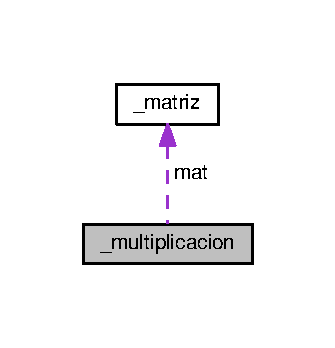
\includegraphics[width=161pt]{struct__multiplicacion__coll__graph}
\end{center}
\end{figure}
\subsection*{Public Attributes}
\begin{DoxyCompactItemize}
\item 
\hyperlink{Ejercicio13_8c_ac63a9b0c7cf4cdbaba641e8f59c29a51}{matriz} \hyperlink{struct__multiplicacion_abfec5d50833a74d0dcc94c685256055f}{mat}
\item 
int {\bfseries multiplicador}\hypertarget{struct__multiplicacion_a97c10b2d4068044f58f4e73a5822c530}{}\label{struct__multiplicacion_a97c10b2d4068044f58f4e73a5822c530}

\item 
int {\bfseries hilo}\hypertarget{struct__multiplicacion_a2143297ffc8eed6a5669b0bf30197371}{}\label{struct__multiplicacion_a2143297ffc8eed6a5669b0bf30197371}

\end{DoxyCompactItemize}


\subsection{Detailed Description}
Estructura para pasar como argumento a los distintos hilos. 

Compuesta por una matriz y un entero que indica el numero de hilo, y otro que indica el numero por el que queremos multiplicar la matriz. 

\subsection{Member Data Documentation}
\index{\+\_\+multiplicacion@{\+\_\+multiplicacion}!mat@{mat}}
\index{mat@{mat}!\+\_\+multiplicacion@{\+\_\+multiplicacion}}
\subsubsection[{\texorpdfstring{mat}{mat}}]{\setlength{\rightskip}{0pt plus 5cm}{\bf matriz} \+\_\+multiplicacion\+::mat}\hypertarget{struct__multiplicacion_abfec5d50833a74d0dcc94c685256055f}{}\label{struct__multiplicacion_abfec5d50833a74d0dcc94c685256055f}
Matriz 

The documentation for this struct was generated from the following files\+:\begin{DoxyCompactItemize}
\item 
\hyperlink{Ejercicio13_8c}{Ejercicio13.\+c}\item 
\hyperlink{Ejercicio13b_8c}{Ejercicio13b.\+c}\end{DoxyCompactItemize}

\chapter{File Documentation}
\hypertarget{Ejercicio12a_8c}{}\section{Ejercicio12a.\+c File Reference}
\label{Ejercicio12a_8c}\index{Ejercicio12a.\+c@{Ejercicio12a.\+c}}


Apartado a del ejercicio 12 Queremos medir el tiempo aproximdo que se tarda en crear y destruir cien procesos, y en que cada uno de estos calcule los N primeros numeros primos, donde N es un parametro introducido por el usuario.  


{\ttfamily \#include $<$stdio.\+h$>$}\\*
{\ttfamily \#include $<$stdlib.\+h$>$}\\*
{\ttfamily \#include $<$string.\+h$>$}\\*
{\ttfamily \#include $<$math.\+h$>$}\\*
{\ttfamily \#include $<$unistd.\+h$>$}\\*
{\ttfamily \#include $<$sys/wait.\+h$>$}\\*
{\ttfamily \#include $<$sys/time.\+h$>$}\\*
{\ttfamily \#include $<$time.\+h$>$}\\*
Include dependency graph for Ejercicio12a.\+c\+:
\nopagebreak
\begin{figure}[H]
\begin{center}
\leavevmode
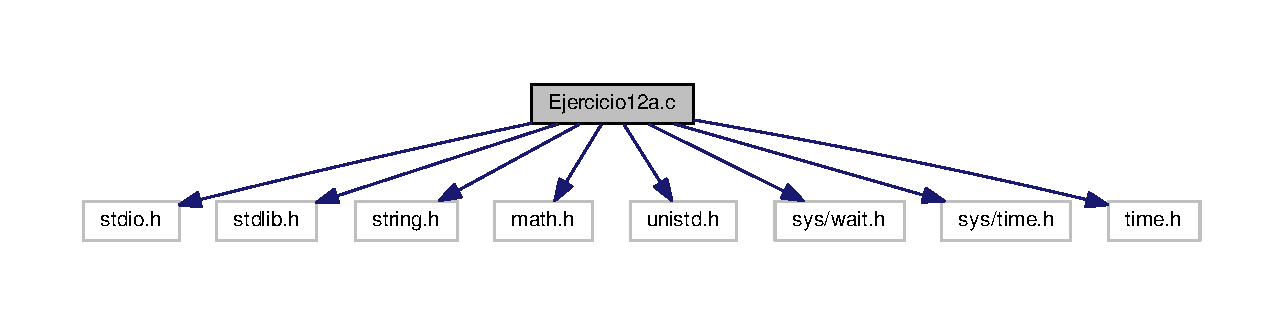
\includegraphics[width=350pt]{Ejercicio12a_8c__incl}
\end{center}
\end{figure}
\subsection*{Classes}
\begin{DoxyCompactItemize}
\item 
struct \hyperlink{struct__estructura}{\+\_\+estructura}
\begin{DoxyCompactList}\small\item\em Estructura para guardar un texto aleatorio y el numero N de primos que tenemos que calcular. \end{DoxyCompactList}\end{DoxyCompactItemize}
\subsection*{Typedefs}
\begin{DoxyCompactItemize}
\item 
typedef struct \hyperlink{struct__estructura}{\+\_\+estructura} \hyperlink{Ejercicio12a_8c_a958d30924884ac1bf0044585c8bc825c}{estructura}
\begin{DoxyCompactList}\small\item\em Estructura para guardar un texto aleatorio y el numero N de primos que tenemos que calcular. \end{DoxyCompactList}\end{DoxyCompactItemize}
\subsection*{Functions}
\begin{DoxyCompactItemize}
\item 
int \hyperlink{Ejercicio12a_8c_ae09682ef27c72bab20d8ab298c7b090f}{es\+\_\+primo} (int n)
\begin{DoxyCompactList}\small\item\em determina si un numero es primo o no. \end{DoxyCompactList}\item 
void $\ast$ \hyperlink{Ejercicio12a_8c_af47ddf18fdd009c7039d7ec241f4d4e5}{calcular\+\_\+primos} (void $\ast$arg)
\begin{DoxyCompactList}\small\item\em calcula todos los primos hasta un N pasado como parte de una estructura estructura. \end{DoxyCompactList}\item 
int \hyperlink{Ejercicio12a_8c_a0ddf1224851353fc92bfbff6f499fa97}{main} (int argc, char $\ast$argv\mbox{[}$\,$\mbox{]})
\begin{DoxyCompactList}\small\item\em crea cien procesos, llama a calcular primos en cada uno de ellos y los espera. \end{DoxyCompactList}\end{DoxyCompactItemize}


\subsection{Detailed Description}
Apartado a del ejercicio 12 Queremos medir el tiempo aproximdo que se tarda en crear y destruir cien procesos, y en que cada uno de estos calcule los N primeros numeros primos, donde N es un parametro introducido por el usuario. 

\begin{DoxyAuthor}{Author}
\href{mailto:Javier.delgadod@estudiante.uam.es}{\tt Javier.\+delgadod@estudiante.\+uam.\+es} \href{mailto:Javier.lopezcano@estudiante.uam.es}{\tt Javier.\+lopezcano@estudiante.\+uam.\+es} 
\end{DoxyAuthor}


\subsection{Typedef Documentation}
\index{Ejercicio12a.\+c@{Ejercicio12a.\+c}!estructura@{estructura}}
\index{estructura@{estructura}!Ejercicio12a.\+c@{Ejercicio12a.\+c}}
\subsubsection[{\texorpdfstring{estructura}{estructura}}]{\setlength{\rightskip}{0pt plus 5cm}typedef struct {\bf \+\_\+estructura} {\bf estructura}}\hypertarget{Ejercicio12a_8c_a958d30924884ac1bf0044585c8bc825c}{}\label{Ejercicio12a_8c_a958d30924884ac1bf0044585c8bc825c}


Estructura para guardar un texto aleatorio y el numero N de primos que tenemos que calcular. 

Compuesta con un string de 100 caracteres y un entero. 

\subsection{Function Documentation}
\index{Ejercicio12a.\+c@{Ejercicio12a.\+c}!calcular\+\_\+primos@{calcular\+\_\+primos}}
\index{calcular\+\_\+primos@{calcular\+\_\+primos}!Ejercicio12a.\+c@{Ejercicio12a.\+c}}
\subsubsection[{\texorpdfstring{calcular\+\_\+primos(void $\ast$arg)}{calcular_primos(void *arg)}}]{\setlength{\rightskip}{0pt plus 5cm}void$\ast$ calcular\+\_\+primos (
\begin{DoxyParamCaption}
\item[{void $\ast$}]{arg}
\end{DoxyParamCaption}
)}\hypertarget{Ejercicio12a_8c_af47ddf18fdd009c7039d7ec241f4d4e5}{}\label{Ejercicio12a_8c_af47ddf18fdd009c7039d7ec241f4d4e5}


calcula todos los primos hasta un N pasado como parte de una estructura estructura. 

\hyperlink{Ejercicio12a_8c_af47ddf18fdd009c7039d7ec241f4d4e5}{calcular\+\_\+primos(void $\ast$arg)} calcula todos los primos hasta un N. 
\begin{DoxyParams}{Parameters}
{\em void} & $\ast$args un puntero a estructura pasado como puntero a void. en el se pasa el numero N. \\
\hline
\end{DoxyParams}
\begin{DoxyReturn}{Returns}
void$\ast$ 0 siempre a N\+U\+LL. 
\end{DoxyReturn}
\index{Ejercicio12a.\+c@{Ejercicio12a.\+c}!es\+\_\+primo@{es\+\_\+primo}}
\index{es\+\_\+primo@{es\+\_\+primo}!Ejercicio12a.\+c@{Ejercicio12a.\+c}}
\subsubsection[{\texorpdfstring{es\+\_\+primo(int n)}{es_primo(int n)}}]{\setlength{\rightskip}{0pt plus 5cm}int es\+\_\+primo (
\begin{DoxyParamCaption}
\item[{int}]{n}
\end{DoxyParamCaption}
)}\hypertarget{Ejercicio12a_8c_ae09682ef27c72bab20d8ab298c7b090f}{}\label{Ejercicio12a_8c_ae09682ef27c72bab20d8ab298c7b090f}


determina si un numero es primo o no. 

\hyperlink{Ejercicio12a_8c_ae09682ef27c72bab20d8ab298c7b090f}{es\+\_\+primo(int n)} determina si n es o no primo. 
\begin{DoxyParams}{Parameters}
{\em n} & numero que queremos saber si es primo. \\
\hline
\end{DoxyParams}
\begin{DoxyReturn}{Returns}
int 0 si no es primo, 1 si si lo es. 
\end{DoxyReturn}
\index{Ejercicio12a.\+c@{Ejercicio12a.\+c}!main@{main}}
\index{main@{main}!Ejercicio12a.\+c@{Ejercicio12a.\+c}}
\subsubsection[{\texorpdfstring{main(int argc, char $\ast$argv[])}{main(int argc, char *argv[])}}]{\setlength{\rightskip}{0pt plus 5cm}int main (
\begin{DoxyParamCaption}
\item[{int}]{argc, }
\item[{char $\ast$}]{argv\mbox{[}$\,$\mbox{]}}
\end{DoxyParamCaption}
)}\hypertarget{Ejercicio12a_8c_a0ddf1224851353fc92bfbff6f499fa97}{}\label{Ejercicio12a_8c_a0ddf1224851353fc92bfbff6f499fa97}


crea cien procesos, llama a calcular primos en cada uno de ellos y los espera. 

main (int argc, char$\ast$ argv\mbox{[}\mbox{]}) cronometra el tiempo que tarda en crear cien procesos que calculan los N primeros primos, donde N se pasa en la entrada, y en destruirlos. Imprime dicho tiempo. 
\begin{DoxyParams}{Parameters}
{\em argc} & numero de argumentos recibidos en la entrada. \\
\hline
{\em argv} & array de strings de argumentos recibidos en la entrada.\\
\hline
\end{DoxyParams}
\begin{DoxyReturn}{Returns}
int que determina si el programa se ha ejecutado o no con exito. 
\end{DoxyReturn}

\hypertarget{Ejercicio12b_8c}{}\section{Ejercicio12b.\+c File Reference}
\label{Ejercicio12b_8c}\index{Ejercicio12b.\+c@{Ejercicio12b.\+c}}


Apartado b del ejercicio 12 Queremos medir el tiempo aproximdo que se tarda en crear y destruir cien hilos, y en que cada uno de estos calcule los N primeros numeros primos, donde N es un parametro introducido por el usuario.  


{\ttfamily \#include $<$stdio.\+h$>$}\\*
{\ttfamily \#include $<$stdlib.\+h$>$}\\*
{\ttfamily \#include $<$string.\+h$>$}\\*
{\ttfamily \#include $<$math.\+h$>$}\\*
{\ttfamily \#include $<$unistd.\+h$>$}\\*
{\ttfamily \#include $<$pthread.\+h$>$}\\*
{\ttfamily \#include $<$sys/time.\+h$>$}\\*
{\ttfamily \#include $<$time.\+h$>$}\\*
Include dependency graph for Ejercicio12b.\+c\+:
\nopagebreak
\begin{figure}[H]
\begin{center}
\leavevmode
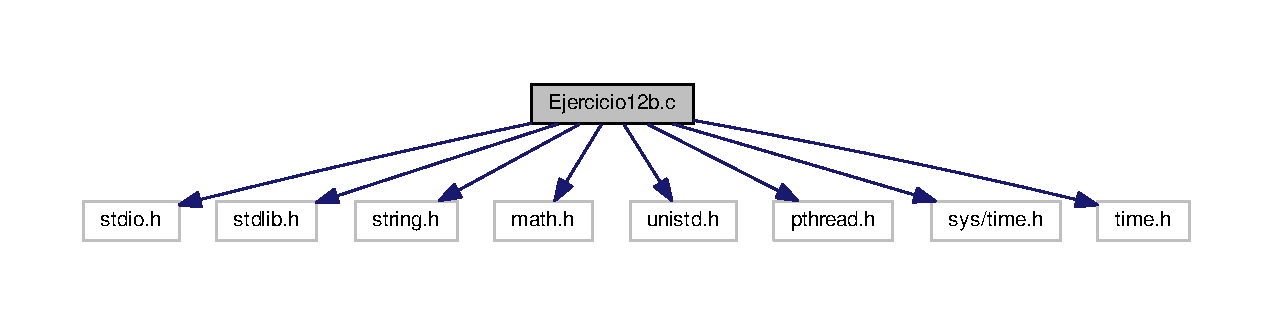
\includegraphics[width=350pt]{Ejercicio12b_8c__incl}
\end{center}
\end{figure}
\subsection*{Classes}
\begin{DoxyCompactItemize}
\item 
struct \hyperlink{struct__estructura}{\+\_\+estructura}
\begin{DoxyCompactList}\small\item\em Estructura para guardar un texto aleatorio y el numero N de primos que tenemos que calcular. \end{DoxyCompactList}\end{DoxyCompactItemize}
\subsection*{Typedefs}
\begin{DoxyCompactItemize}
\item 
typedef struct \hyperlink{struct__estructura}{\+\_\+estructura} \hyperlink{Ejercicio12b_8c_a958d30924884ac1bf0044585c8bc825c}{estructura}
\begin{DoxyCompactList}\small\item\em Estructura para guardar un texto aleatorio y el numero N de primos que tenemos que calcular. \end{DoxyCompactList}\end{DoxyCompactItemize}
\subsection*{Functions}
\begin{DoxyCompactItemize}
\item 
int \hyperlink{Ejercicio12b_8c_ae09682ef27c72bab20d8ab298c7b090f}{es\+\_\+primo} (int n)
\begin{DoxyCompactList}\small\item\em determina si un numero es primo o no. \end{DoxyCompactList}\item 
void $\ast$ \hyperlink{Ejercicio12b_8c_af47ddf18fdd009c7039d7ec241f4d4e5}{calcular\+\_\+primos} (void $\ast$arg)
\begin{DoxyCompactList}\small\item\em calcula todos los primos hasta un N pasado como parte de una estructura estructura. \end{DoxyCompactList}\item 
int \hyperlink{Ejercicio12b_8c_a0ddf1224851353fc92bfbff6f499fa97}{main} (int argc, char $\ast$argv\mbox{[}$\,$\mbox{]})
\begin{DoxyCompactList}\small\item\em crea cien hilos, llama a calcular primos en cad uno de ellos y los espera. \end{DoxyCompactList}\end{DoxyCompactItemize}


\subsection{Detailed Description}
Apartado b del ejercicio 12 Queremos medir el tiempo aproximdo que se tarda en crear y destruir cien hilos, y en que cada uno de estos calcule los N primeros numeros primos, donde N es un parametro introducido por el usuario. 

\begin{DoxyAuthor}{Author}
\href{mailto:Javier.delgadod@estudiante.uam.es}{\tt Javier.\+delgadod@estudiante.\+uam.\+es} \href{mailto:Javier.lopezcano@estudiante.uam.es}{\tt Javier.\+lopezcano@estudiante.\+uam.\+es} 
\end{DoxyAuthor}


\subsection{Typedef Documentation}
\index{Ejercicio12b.\+c@{Ejercicio12b.\+c}!estructura@{estructura}}
\index{estructura@{estructura}!Ejercicio12b.\+c@{Ejercicio12b.\+c}}
\subsubsection[{\texorpdfstring{estructura}{estructura}}]{\setlength{\rightskip}{0pt plus 5cm}typedef struct {\bf \+\_\+estructura} {\bf estructura}}\hypertarget{Ejercicio12b_8c_a958d30924884ac1bf0044585c8bc825c}{}\label{Ejercicio12b_8c_a958d30924884ac1bf0044585c8bc825c}


Estructura para guardar un texto aleatorio y el numero N de primos que tenemos que calcular. 

Compuesta con un string de 100 caracteres y un entero. 

\subsection{Function Documentation}
\index{Ejercicio12b.\+c@{Ejercicio12b.\+c}!calcular\+\_\+primos@{calcular\+\_\+primos}}
\index{calcular\+\_\+primos@{calcular\+\_\+primos}!Ejercicio12b.\+c@{Ejercicio12b.\+c}}
\subsubsection[{\texorpdfstring{calcular\+\_\+primos(void $\ast$arg)}{calcular_primos(void *arg)}}]{\setlength{\rightskip}{0pt plus 5cm}void$\ast$ calcular\+\_\+primos (
\begin{DoxyParamCaption}
\item[{void $\ast$}]{arg}
\end{DoxyParamCaption}
)}\hypertarget{Ejercicio12b_8c_af47ddf18fdd009c7039d7ec241f4d4e5}{}\label{Ejercicio12b_8c_af47ddf18fdd009c7039d7ec241f4d4e5}


calcula todos los primos hasta un N pasado como parte de una estructura estructura. 

\hyperlink{Ejercicio12b_8c_af47ddf18fdd009c7039d7ec241f4d4e5}{calcular\+\_\+primos(void $\ast$arg)} calcula todos los primos hasta un N. 
\begin{DoxyParams}{Parameters}
{\em void} & $\ast$args un puntero a estructura pasado como puntero a void. en el se pasa el numero N. \\
\hline
\end{DoxyParams}
\begin{DoxyReturn}{Returns}
void$\ast$ 0 siempre a N\+U\+LL. 
\end{DoxyReturn}
\index{Ejercicio12b.\+c@{Ejercicio12b.\+c}!es\+\_\+primo@{es\+\_\+primo}}
\index{es\+\_\+primo@{es\+\_\+primo}!Ejercicio12b.\+c@{Ejercicio12b.\+c}}
\subsubsection[{\texorpdfstring{es\+\_\+primo(int n)}{es_primo(int n)}}]{\setlength{\rightskip}{0pt plus 5cm}int es\+\_\+primo (
\begin{DoxyParamCaption}
\item[{int}]{n}
\end{DoxyParamCaption}
)}\hypertarget{Ejercicio12b_8c_ae09682ef27c72bab20d8ab298c7b090f}{}\label{Ejercicio12b_8c_ae09682ef27c72bab20d8ab298c7b090f}


determina si un numero es primo o no. 

\hyperlink{Ejercicio12b_8c_ae09682ef27c72bab20d8ab298c7b090f}{es\+\_\+primo(int n)} determina si n es o no primo. 
\begin{DoxyParams}{Parameters}
{\em n} & numero que queremos saber si es primo. \\
\hline
\end{DoxyParams}
\begin{DoxyReturn}{Returns}
int 0 si no es primo, 1 si si lo es. 
\end{DoxyReturn}
\index{Ejercicio12b.\+c@{Ejercicio12b.\+c}!main@{main}}
\index{main@{main}!Ejercicio12b.\+c@{Ejercicio12b.\+c}}
\subsubsection[{\texorpdfstring{main(int argc, char $\ast$argv[])}{main(int argc, char *argv[])}}]{\setlength{\rightskip}{0pt plus 5cm}int main (
\begin{DoxyParamCaption}
\item[{int}]{argc, }
\item[{char $\ast$}]{argv\mbox{[}$\,$\mbox{]}}
\end{DoxyParamCaption}
)}\hypertarget{Ejercicio12b_8c_a0ddf1224851353fc92bfbff6f499fa97}{}\label{Ejercicio12b_8c_a0ddf1224851353fc92bfbff6f499fa97}


crea cien hilos, llama a calcular primos en cad uno de ellos y los espera. 

main (int argc, char$\ast$ argv\mbox{[}\mbox{]}) cronometra el tiempo que tarda en crear cien hilos que calculan los N primeros primos, donde N se pasa en la entrada, y en destruirlos. Imprime dicho tiempo. 
\begin{DoxyParams}{Parameters}
{\em argc} & numero de argumentos recibidos en la entrada. \\
\hline
{\em argv} & array de strings de argumentos recibidos en la entrada.\\
\hline
\end{DoxyParams}
\begin{DoxyReturn}{Returns}
int que determina si el programa se ha ejecutado o no con exito. 
\end{DoxyReturn}

\hypertarget{Ejercicio13_8c}{}\section{Ejercicio13.\+c File Reference}
\label{Ejercicio13_8c}\index{Ejercicio13.\+c@{Ejercicio13.\+c}}


Ejercicio 13 Queremos crear dos hilos para que multipliquen simultaneamente una matriz por un entero cada uno.  


{\ttfamily \#include $<$stdio.\+h$>$}\\*
{\ttfamily \#include $<$stdlib.\+h$>$}\\*
{\ttfamily \#include $<$string.\+h$>$}\\*
{\ttfamily \#include $<$unistd.\+h$>$}\\*
{\ttfamily \#include $<$pthread.\+h$>$}\\*
Include dependency graph for Ejercicio13.\+c\+:
\nopagebreak
\begin{figure}[H]
\begin{center}
\leavevmode
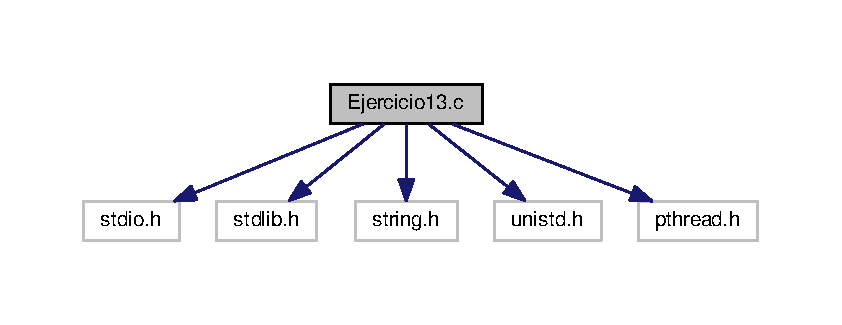
\includegraphics[width=350pt]{Ejercicio13_8c__incl}
\end{center}
\end{figure}
\subsection*{Classes}
\begin{DoxyCompactItemize}
\item 
struct \hyperlink{struct__matriz}{\+\_\+matriz}
\begin{DoxyCompactList}\small\item\em Estructura para representar una matriz cuadrada de hasta cinco por cinco enteros. \end{DoxyCompactList}\item 
struct \hyperlink{struct__multiplicacion}{\+\_\+multiplicacion}
\begin{DoxyCompactList}\small\item\em Estructura para pasar como argumento a los distintos hilos. \end{DoxyCompactList}\end{DoxyCompactItemize}
\subsection*{Typedefs}
\begin{DoxyCompactItemize}
\item 
typedef struct \hyperlink{struct__matriz}{\+\_\+matriz} \hyperlink{Ejercicio13_8c_ac63a9b0c7cf4cdbaba641e8f59c29a51}{matriz}
\begin{DoxyCompactList}\small\item\em Estructura para representar una matriz cuadrada de hasta cinco por cinco enteros. \end{DoxyCompactList}\item 
typedef struct \hyperlink{struct__multiplicacion}{\+\_\+multiplicacion} \hyperlink{Ejercicio13_8c_ad1b3bf648d6b4a06bc703025cce83b58}{multiplicacion}
\begin{DoxyCompactList}\small\item\em Estructura para pasar como argumento a los distintos hilos. \end{DoxyCompactList}\end{DoxyCompactItemize}
\subsection*{Functions}
\begin{DoxyCompactItemize}
\item 
void $\ast$ \hyperlink{Ejercicio13_8c_a897014abd1504939e716e633e68d2788}{multiplicar\+Matriz} (void $\ast$args)
\begin{DoxyCompactList}\small\item\em multiplica una matriz cuadrada por un entero. \end{DoxyCompactList}\item 
int \hyperlink{Ejercicio13_8c_a0ddf1224851353fc92bfbff6f499fa97}{main} (int argc, char $\ast$argv\mbox{[}$\,$\mbox{]})
\begin{DoxyCompactList}\small\item\em crea dos hilos para multiplicar dos matrices por dos enteros respectivamente. \end{DoxyCompactList}\end{DoxyCompactItemize}


\subsection{Detailed Description}
Ejercicio 13 Queremos crear dos hilos para que multipliquen simultaneamente una matriz por un entero cada uno. 

\begin{DoxyAuthor}{Author}
\href{mailto:Javier.delgadod@estudiante.uam.es}{\tt Javier.\+delgadod@estudiante.\+uam.\+es} \href{mailto:Javier.lopezcano@estudiante.uam.es}{\tt Javier.\+lopezcano@estudiante.\+uam.\+es} 
\end{DoxyAuthor}


\subsection{Typedef Documentation}
\index{Ejercicio13.\+c@{Ejercicio13.\+c}!matriz@{matriz}}
\index{matriz@{matriz}!Ejercicio13.\+c@{Ejercicio13.\+c}}
\subsubsection[{\texorpdfstring{matriz}{matriz}}]{\setlength{\rightskip}{0pt plus 5cm}typedef struct {\bf \+\_\+matriz} {\bf matriz}}\hypertarget{Ejercicio13_8c_ac63a9b0c7cf4cdbaba641e8f59c29a51}{}\label{Ejercicio13_8c_ac63a9b0c7cf4cdbaba641e8f59c29a51}


Estructura para representar una matriz cuadrada de hasta cinco por cinco enteros. 

Compuesta por un doble array y un entero que indica su tamaño. \index{Ejercicio13.\+c@{Ejercicio13.\+c}!multiplicacion@{multiplicacion}}
\index{multiplicacion@{multiplicacion}!Ejercicio13.\+c@{Ejercicio13.\+c}}
\subsubsection[{\texorpdfstring{multiplicacion}{multiplicacion}}]{\setlength{\rightskip}{0pt plus 5cm}typedef struct {\bf \+\_\+multiplicacion} {\bf multiplicacion}}\hypertarget{Ejercicio13_8c_ad1b3bf648d6b4a06bc703025cce83b58}{}\label{Ejercicio13_8c_ad1b3bf648d6b4a06bc703025cce83b58}


Estructura para pasar como argumento a los distintos hilos. 

Compuesta por una matriz y un entero que indica el numero de hilo, y otro que indica el numero por el que queremos multiplicar la matriz. 

\subsection{Function Documentation}
\index{Ejercicio13.\+c@{Ejercicio13.\+c}!main@{main}}
\index{main@{main}!Ejercicio13.\+c@{Ejercicio13.\+c}}
\subsubsection[{\texorpdfstring{main(int argc, char $\ast$argv[])}{main(int argc, char *argv[])}}]{\setlength{\rightskip}{0pt plus 5cm}int main (
\begin{DoxyParamCaption}
\item[{int}]{argc, }
\item[{char $\ast$}]{argv\mbox{[}$\,$\mbox{]}}
\end{DoxyParamCaption}
)}\hypertarget{Ejercicio13_8c_a0ddf1224851353fc92bfbff6f499fa97}{}\label{Ejercicio13_8c_a0ddf1224851353fc92bfbff6f499fa97}


crea dos hilos para multiplicar dos matrices por dos enteros respectivamente. 

main (int argc, char$\ast$ argv\mbox{[}\mbox{]}) obtiene dos matrices cuadradas y dos multiplicadores mediante la entrada del teclado, y crea un hilo para mutiplicar cada una de estas matrices por el multiplicador. 
\begin{DoxyParams}{Parameters}
{\em argc} & numero de argumentos recibidos en la entrada. \\
\hline
{\em argv} & array de strings de argumentos recibidos en la entrada.\\
\hline
\end{DoxyParams}
\begin{DoxyReturn}{Returns}
int que determina si el programa se ha ejecutado o no con exito. 
\end{DoxyReturn}
\index{Ejercicio13.\+c@{Ejercicio13.\+c}!multiplicar\+Matriz@{multiplicar\+Matriz}}
\index{multiplicar\+Matriz@{multiplicar\+Matriz}!Ejercicio13.\+c@{Ejercicio13.\+c}}
\subsubsection[{\texorpdfstring{multiplicar\+Matriz(void $\ast$args)}{multiplicarMatriz(void *args)}}]{\setlength{\rightskip}{0pt plus 5cm}void$\ast$ multiplicar\+Matriz (
\begin{DoxyParamCaption}
\item[{void $\ast$}]{args}
\end{DoxyParamCaption}
)}\hypertarget{Ejercicio13_8c_a897014abd1504939e716e633e68d2788}{}\label{Ejercicio13_8c_a897014abd1504939e716e633e68d2788}


multiplica una matriz cuadrada por un entero. 

\hyperlink{Ejercicio13_8c_a897014abd1504939e716e633e68d2788}{multiplicar\+Matriz(void $\ast$args)} mutiplica una matriz por un numero fila por fila, imprimiendo el resultado y el numero del hilo.


\begin{DoxyParams}{Parameters}
{\em args} & un puntero a multiplicacion pasado como puntero a void. en el se pasa la matriz y el multiplicador. \\
\hline
\end{DoxyParams}
\begin{DoxyReturn}{Returns}
void$\ast$ 0 siempre a N\+U\+LL. 
\end{DoxyReturn}

\hypertarget{Ejercicio13b_8c}{}\section{Ejercicio13b.\+c File Reference}
\label{Ejercicio13b_8c}\index{Ejercicio13b.\+c@{Ejercicio13b.\+c}}


Ejercicio 13b Queremos crear dos hilos para que multipliquen simultaneamente una matriz por un entero cada uno, y que se comuniquen usando variables globales de forma que cada hilo sepa por donde va el otro.  


{\ttfamily \#include $<$stdio.\+h$>$}\\*
{\ttfamily \#include $<$stdlib.\+h$>$}\\*
{\ttfamily \#include $<$string.\+h$>$}\\*
{\ttfamily \#include $<$math.\+h$>$}\\*
{\ttfamily \#include $<$unistd.\+h$>$}\\*
{\ttfamily \#include $<$time.\+h$>$}\\*
{\ttfamily \#include $<$pthread.\+h$>$}\\*
Include dependency graph for Ejercicio13b.\+c\+:
\nopagebreak
\begin{figure}[H]
\begin{center}
\leavevmode
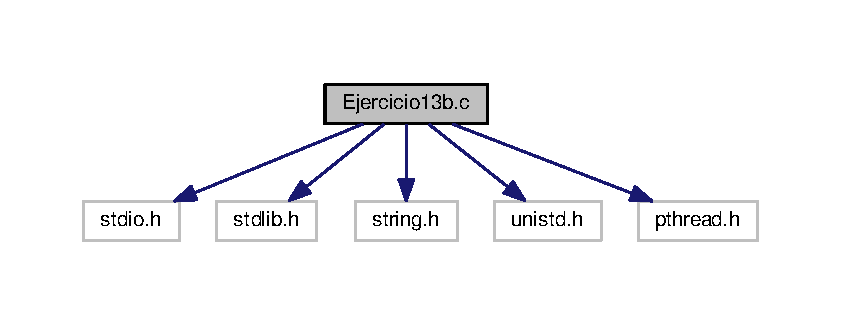
\includegraphics[width=350pt]{Ejercicio13b_8c__incl}
\end{center}
\end{figure}
\subsection*{Classes}
\begin{DoxyCompactItemize}
\item 
struct \hyperlink{struct__matriz}{\+\_\+matriz}
\begin{DoxyCompactList}\small\item\em Estructura para representar una matriz cuadrada de hasta cinco por cinco enteros. \end{DoxyCompactList}\item 
struct \hyperlink{struct__multiplicacion}{\+\_\+multiplicacion}
\begin{DoxyCompactList}\small\item\em Estructura para pasar como argumento a los distintos hilos. \end{DoxyCompactList}\end{DoxyCompactItemize}
\subsection*{Typedefs}
\begin{DoxyCompactItemize}
\item 
typedef struct \hyperlink{struct__matriz}{\+\_\+matriz} \hyperlink{Ejercicio13b_8c_ac63a9b0c7cf4cdbaba641e8f59c29a51}{matriz}
\begin{DoxyCompactList}\small\item\em Estructura para representar una matriz cuadrada de hasta cinco por cinco enteros. \end{DoxyCompactList}\item 
typedef struct \hyperlink{struct__multiplicacion}{\+\_\+multiplicacion} \hyperlink{Ejercicio13b_8c_ad1b3bf648d6b4a06bc703025cce83b58}{multiplicacion}
\begin{DoxyCompactList}\small\item\em Estructura para pasar como argumento a los distintos hilos. \end{DoxyCompactList}\end{DoxyCompactItemize}
\subsection*{Functions}
\begin{DoxyCompactItemize}
\item 
void $\ast$ \hyperlink{Ejercicio13b_8c_a897014abd1504939e716e633e68d2788}{multiplicar\+Matriz} (void $\ast$args)
\begin{DoxyCompactList}\small\item\em multiplica una matriz cuadrada por un entero. \end{DoxyCompactList}\item 
int \hyperlink{Ejercicio13b_8c_a0ddf1224851353fc92bfbff6f499fa97}{main} (int argc, char $\ast$argv\mbox{[}$\,$\mbox{]})
\begin{DoxyCompactList}\small\item\em crea dos hilos para multiplicar dos matrices por dos enteros respectivamente. \end{DoxyCompactList}\end{DoxyCompactItemize}
\subsection*{Variables}
\begin{DoxyCompactItemize}
\item 
int {\bfseries pos1}\hypertarget{Ejercicio13b_8c_a363774778a5ad0ef78e6e4ca79a3bc11}{}\label{Ejercicio13b_8c_a363774778a5ad0ef78e6e4ca79a3bc11}

\item 
int \hyperlink{Ejercicio13b_8c_a1b3a85917a11704027ecd416ffa736fc}{pos2}
\end{DoxyCompactItemize}


\subsection{Detailed Description}
Ejercicio 13b Queremos crear dos hilos para que multipliquen simultaneamente una matriz por un entero cada uno, y que se comuniquen usando variables globales de forma que cada hilo sepa por donde va el otro. 

\begin{DoxyAuthor}{Author}
\href{mailto:Javier.delgadod@estudiante.uam.es}{\tt Javier.\+delgadod@estudiante.\+uam.\+es} \href{mailto:Javier.lopezcano@estudiante.uam.es}{\tt Javier.\+lopezcano@estudiante.\+uam.\+es} 
\end{DoxyAuthor}


\subsection{Typedef Documentation}
\index{Ejercicio13b.\+c@{Ejercicio13b.\+c}!matriz@{matriz}}
\index{matriz@{matriz}!Ejercicio13b.\+c@{Ejercicio13b.\+c}}
\subsubsection[{\texorpdfstring{matriz}{matriz}}]{\setlength{\rightskip}{0pt plus 5cm}typedef struct {\bf \+\_\+matriz} {\bf matriz}}\hypertarget{Ejercicio13b_8c_ac63a9b0c7cf4cdbaba641e8f59c29a51}{}\label{Ejercicio13b_8c_ac63a9b0c7cf4cdbaba641e8f59c29a51}


Estructura para representar una matriz cuadrada de hasta cinco por cinco enteros. 

Compuesta por un doble array y un entero que indica su tamaño. \index{Ejercicio13b.\+c@{Ejercicio13b.\+c}!multiplicacion@{multiplicacion}}
\index{multiplicacion@{multiplicacion}!Ejercicio13b.\+c@{Ejercicio13b.\+c}}
\subsubsection[{\texorpdfstring{multiplicacion}{multiplicacion}}]{\setlength{\rightskip}{0pt plus 5cm}typedef struct {\bf \+\_\+multiplicacion} {\bf multiplicacion}}\hypertarget{Ejercicio13b_8c_ad1b3bf648d6b4a06bc703025cce83b58}{}\label{Ejercicio13b_8c_ad1b3bf648d6b4a06bc703025cce83b58}


Estructura para pasar como argumento a los distintos hilos. 

Compuesta por una matriz y un entero que indica el numero de hilo, y otro que indica el numero por el que queremos multiplicar la matriz. 

\subsection{Function Documentation}
\index{Ejercicio13b.\+c@{Ejercicio13b.\+c}!main@{main}}
\index{main@{main}!Ejercicio13b.\+c@{Ejercicio13b.\+c}}
\subsubsection[{\texorpdfstring{main(int argc, char $\ast$argv[])}{main(int argc, char *argv[])}}]{\setlength{\rightskip}{0pt plus 5cm}int main (
\begin{DoxyParamCaption}
\item[{int}]{argc, }
\item[{char $\ast$}]{argv\mbox{[}$\,$\mbox{]}}
\end{DoxyParamCaption}
)}\hypertarget{Ejercicio13b_8c_a0ddf1224851353fc92bfbff6f499fa97}{}\label{Ejercicio13b_8c_a0ddf1224851353fc92bfbff6f499fa97}


crea dos hilos para multiplicar dos matrices por dos enteros respectivamente. 

main (int argc, char$\ast$ argv\mbox{[}\mbox{]}) obtiene dos matrices cuadradas y dos multiplicadores mediante la entrada del teclado, y crea un hilo para mutiplicar cada una de estas matrices por el multiplicador. 
\begin{DoxyParams}{Parameters}
{\em argc} & numero de argumentos recibidos en la entrada. \\
\hline
{\em argv} & array de strings de argumentos recibidos en la entrada.\\
\hline
\end{DoxyParams}
\begin{DoxyReturn}{Returns}
int que determina si el programa se ha ejecutado o no con exito. 
\end{DoxyReturn}
\index{Ejercicio13b.\+c@{Ejercicio13b.\+c}!multiplicar\+Matriz@{multiplicar\+Matriz}}
\index{multiplicar\+Matriz@{multiplicar\+Matriz}!Ejercicio13b.\+c@{Ejercicio13b.\+c}}
\subsubsection[{\texorpdfstring{multiplicar\+Matriz(void $\ast$args)}{multiplicarMatriz(void *args)}}]{\setlength{\rightskip}{0pt plus 5cm}void$\ast$ multiplicar\+Matriz (
\begin{DoxyParamCaption}
\item[{void $\ast$}]{args}
\end{DoxyParamCaption}
)}\hypertarget{Ejercicio13b_8c_a897014abd1504939e716e633e68d2788}{}\label{Ejercicio13b_8c_a897014abd1504939e716e633e68d2788}


multiplica una matriz cuadrada por un entero. 

\hyperlink{Ejercicio13b_8c_a897014abd1504939e716e633e68d2788}{multiplicar\+Matriz(void $\ast$args)} mutiplica una matriz por un numero fila por fila, imprimiendo el resultado y el numero del hilo.


\begin{DoxyParams}{Parameters}
{\em args} & un puntero a multiplicacion pasado como puntero a void. en el se pasa la matriz y el multiplicador. \\
\hline
\end{DoxyParams}
\begin{DoxyReturn}{Returns}
void$\ast$ 0 siempre a N\+U\+LL. 
\end{DoxyReturn}


\subsection{Variable Documentation}
\index{Ejercicio13b.\+c@{Ejercicio13b.\+c}!pos2@{pos2}}
\index{pos2@{pos2}!Ejercicio13b.\+c@{Ejercicio13b.\+c}}
\subsubsection[{\texorpdfstring{pos2}{pos2}}]{\setlength{\rightskip}{0pt plus 5cm}int pos2}\hypertarget{Ejercicio13b_8c_a1b3a85917a11704027ecd416ffa736fc}{}\label{Ejercicio13b_8c_a1b3a85917a11704027ecd416ffa736fc}
Variables globales usadas para la comunicacion entre hilos 
\hypertarget{Ejercicio4_8c}{}\section{Ejercicio4.\+c File Reference}
\label{Ejercicio4_8c}\index{Ejercicio4.\+c@{Ejercicio4.\+c}}


Ejercicio 4 de la Practica 2.  


{\ttfamily \#include $<$stdio.\+h$>$}\\*
{\ttfamily \#include $<$sys/types.\+h$>$}\\*
{\ttfamily \#include $<$sys/wait.\+h$>$}\\*
{\ttfamily \#include $<$stdlib.\+h$>$}\\*
{\ttfamily \#include $<$unistd.\+h$>$}\\*
{\ttfamily \#include $<$signal.\+h$>$}\\*
Include dependency graph for Ejercicio4.\+c\+:
\nopagebreak
\begin{figure}[H]
\begin{center}
\leavevmode
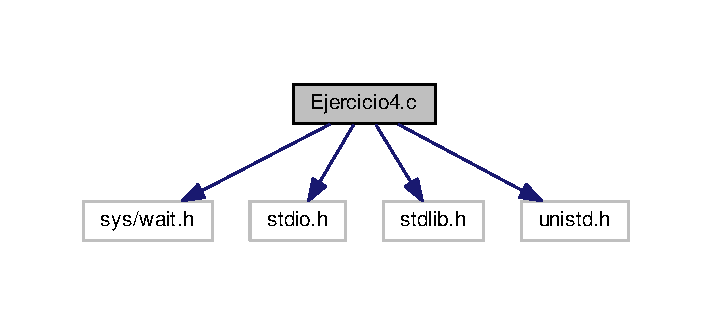
\includegraphics[width=350pt]{Ejercicio4_8c__incl}
\end{center}
\end{figure}
\subsection*{Macros}
\begin{DoxyCompactItemize}
\item 
\#define \hyperlink{Ejercicio4_8c_a9dd395f2e0046c1513c84dfcfb9e54da}{N\+U\+M\+\_\+\+H\+I\+J\+OS}~5
\end{DoxyCompactItemize}
\subsection*{Functions}
\begin{DoxyCompactItemize}
\item 
void \hyperlink{Ejercicio4_8c_a0897883a0dfdf1023f377e262cee1299}{captura} ()\hypertarget{Ejercicio4_8c_a0897883a0dfdf1023f377e262cee1299}{}\label{Ejercicio4_8c_a0897883a0dfdf1023f377e262cee1299}

\begin{DoxyCompactList}\small\item\em Funcion que ejecuta el proceso padre tras recibir la senal S\+I\+G\+U\+S\+R1. De esta forma, nos aseguramos que el proceso salga correctamente del pause() y continue su ejecucion. \end{DoxyCompactList}\item 
void \hyperlink{Ejercicio4_8c_a8dde52fc2d8703ce2fa56ebedcacee05}{terminar} ()\hypertarget{Ejercicio4_8c_a8dde52fc2d8703ce2fa56ebedcacee05}{}\label{Ejercicio4_8c_a8dde52fc2d8703ce2fa56ebedcacee05}

\begin{DoxyCompactList}\small\item\em Funcion que ejecutan los procesos hijos tras recibir la senal S\+I\+G\+U\+S\+R2, para terminar asi su ejecucion. \end{DoxyCompactList}\item 
int \hyperlink{Ejercicio4_8c_ae66f6b31b5ad750f1fe042a706a4e3d4}{main} ()
\begin{DoxyCompactList}\small\item\em El proceso padre crea un proceso hijo, que imprime 10 veces \char`\"{}\+Soy $<$\+P\+I\+D$>$ y estoy trabajando\char`\"{}, esperando un segundo entre cada vez. Una vez el proceso hijo ha impreso el texto las 10 veces, manda la señal S\+I\+G\+U\+S\+R1 al padre, que sale del pause(), y crea otro hijo, de forma que es este nuevo hijo el que manda una senal S\+I\+G\+U\+S\+R2 al hijo anterior para que este se termine a el mismo. Asi, el padre acaba creando N\+U\+M\+\_\+\+H\+I\+J\+OS procesos hijos, el mismo mata al ultimo de los hijos, y se asegura de esperar a todos. \end{DoxyCompactList}\end{DoxyCompactItemize}


\subsection{Detailed Description}
Ejercicio 4 de la Practica 2. 

\begin{DoxyAuthor}{Author}
\href{mailto:Javier.delgadod@estudiante.uam.es}{\tt Javier.\+delgadod@estudiante.\+uam.\+es} 

\href{mailto:Javier.lopezcano@estudiante.uam.es}{\tt Javier.\+lopezcano@estudiante.\+uam.\+es} 
\end{DoxyAuthor}


\subsection{Macro Definition Documentation}
\index{Ejercicio4.\+c@{Ejercicio4.\+c}!N\+U\+M\+\_\+\+H\+I\+J\+OS@{N\+U\+M\+\_\+\+H\+I\+J\+OS}}
\index{N\+U\+M\+\_\+\+H\+I\+J\+OS@{N\+U\+M\+\_\+\+H\+I\+J\+OS}!Ejercicio4.\+c@{Ejercicio4.\+c}}
\subsubsection[{\texorpdfstring{N\+U\+M\+\_\+\+H\+I\+J\+OS}{NUM_HIJOS}}]{\setlength{\rightskip}{0pt plus 5cm}\#define N\+U\+M\+\_\+\+H\+I\+J\+OS~5}\hypertarget{Ejercicio4_8c_a9dd395f2e0046c1513c84dfcfb9e54da}{}\label{Ejercicio4_8c_a9dd395f2e0046c1513c84dfcfb9e54da}
Numero de hijos que crea el proceso padre 

\subsection{Function Documentation}
\index{Ejercicio4.\+c@{Ejercicio4.\+c}!main@{main}}
\index{main@{main}!Ejercicio4.\+c@{Ejercicio4.\+c}}
\subsubsection[{\texorpdfstring{main()}{main()}}]{\setlength{\rightskip}{0pt plus 5cm}int main (
\begin{DoxyParamCaption}
\item[{void}]{}
\end{DoxyParamCaption}
)}\hypertarget{Ejercicio4_8c_ae66f6b31b5ad750f1fe042a706a4e3d4}{}\label{Ejercicio4_8c_ae66f6b31b5ad750f1fe042a706a4e3d4}


El proceso padre crea un proceso hijo, que imprime 10 veces \char`\"{}\+Soy $<$\+P\+I\+D$>$ y estoy trabajando\char`\"{}, esperando un segundo entre cada vez. Una vez el proceso hijo ha impreso el texto las 10 veces, manda la señal S\+I\+G\+U\+S\+R1 al padre, que sale del pause(), y crea otro hijo, de forma que es este nuevo hijo el que manda una senal S\+I\+G\+U\+S\+R2 al hijo anterior para que este se termine a el mismo. Asi, el padre acaba creando N\+U\+M\+\_\+\+H\+I\+J\+OS procesos hijos, el mismo mata al ultimo de los hijos, y se asegura de esperar a todos. 

\begin{DoxyReturn}{Returns}
int que determina si el programa se ha ejecutado o no con exito. 
\end{DoxyReturn}

\hypertarget{Ejercicio5a_8c}{}\section{Ejercicio5a.\+c File Reference}
\label{Ejercicio5a_8c}\index{Ejercicio5a.\+c@{Ejercicio5a.\+c}}


Apartado a del ejercicio 5. Modificamos el ejercicio 4 minimamentepara que se generen procesos para los numeros i impares, de forma que cada padre tiene un unico hijo y le tiene que esperar.  


{\ttfamily \#include $<$sys/wait.\+h$>$}\\*
{\ttfamily \#include $<$stdio.\+h$>$}\\*
{\ttfamily \#include $<$stdlib.\+h$>$}\\*
{\ttfamily \#include $<$unistd.\+h$>$}\\*
Include dependency graph for Ejercicio5a.\+c\+:
\nopagebreak
\begin{figure}[H]
\begin{center}
\leavevmode
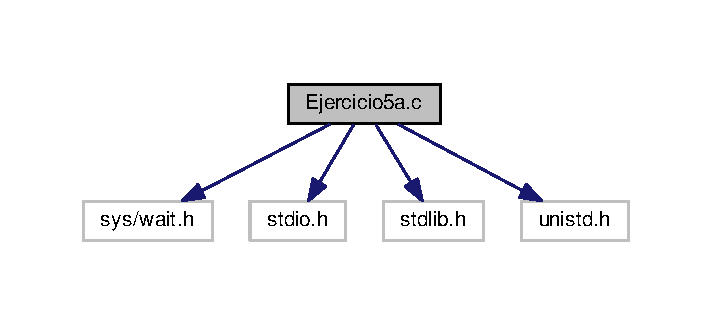
\includegraphics[width=342pt]{Ejercicio5a_8c__incl}
\end{center}
\end{figure}
\subsection*{Macros}
\begin{DoxyCompactItemize}
\item 
\#define \hyperlink{Ejercicio5a_8c_acee2369f62e4a096d243dec3cd7d0b00}{N\+U\+M\+\_\+\+P\+R\+OC}~6
\end{DoxyCompactItemize}
\subsection*{Functions}
\begin{DoxyCompactItemize}
\item 
int \hyperlink{Ejercicio5a_8c_ae66f6b31b5ad750f1fe042a706a4e3d4}{main} ()\hypertarget{Ejercicio5a_8c_ae66f6b31b5ad750f1fe042a706a4e3d4}{}\label{Ejercicio5a_8c_ae66f6b31b5ad750f1fe042a706a4e3d4}

\begin{DoxyCompactList}\small\item\em Crea un arbol de procesos de forma que cada proceso crea un unico hijo, y se asegura de esperarle. \end{DoxyCompactList}\end{DoxyCompactItemize}


\subsection{Detailed Description}
Apartado a del ejercicio 5. Modificamos el ejercicio 4 minimamentepara que se generen procesos para los numeros i impares, de forma que cada padre tiene un unico hijo y le tiene que esperar. 

\begin{DoxyAuthor}{Author}
\href{mailto:Javier.delgadod@estudiante.uam.es}{\tt Javier.\+delgadod@estudiante.\+uam.\+es} \href{mailto:Javier.lopezcano@estudiante.uam.es}{\tt Javier.\+lopezcano@estudiante.\+uam.\+es} 
\end{DoxyAuthor}


\subsection{Macro Definition Documentation}
\index{Ejercicio5a.\+c@{Ejercicio5a.\+c}!N\+U\+M\+\_\+\+P\+R\+OC@{N\+U\+M\+\_\+\+P\+R\+OC}}
\index{N\+U\+M\+\_\+\+P\+R\+OC@{N\+U\+M\+\_\+\+P\+R\+OC}!Ejercicio5a.\+c@{Ejercicio5a.\+c}}
\subsubsection[{\texorpdfstring{N\+U\+M\+\_\+\+P\+R\+OC}{NUM_PROC}}]{\setlength{\rightskip}{0pt plus 5cm}\#define N\+U\+M\+\_\+\+P\+R\+OC~6}\hypertarget{Ejercicio5a_8c_acee2369f62e4a096d243dec3cd7d0b00}{}\label{Ejercicio5a_8c_acee2369f62e4a096d243dec3cd7d0b00}
Numero de veces que se recorre el bucle 
\hypertarget{Ejercicio5b_8c}{}\section{Ejercicio5b.\+c File Reference}
\label{Ejercicio5b_8c}\index{Ejercicio5b.\+c@{Ejercicio5b.\+c}}


Apartado a del ejercicio 5. Modificamos el ejercicio 4 minimamentepara que el proceso padre genere hijos para los numeros i impares y los espere.  


{\ttfamily \#include $<$sys/wait.\+h$>$}\\*
{\ttfamily \#include $<$stdio.\+h$>$}\\*
{\ttfamily \#include $<$stdlib.\+h$>$}\\*
{\ttfamily \#include $<$unistd.\+h$>$}\\*
Include dependency graph for Ejercicio5b.\+c\+:
\nopagebreak
\begin{figure}[H]
\begin{center}
\leavevmode
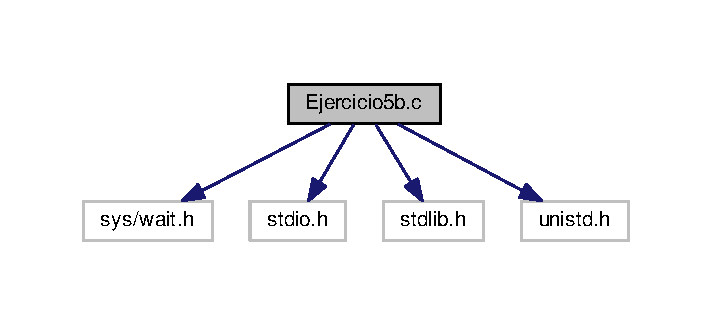
\includegraphics[width=342pt]{Ejercicio5b_8c__incl}
\end{center}
\end{figure}
\subsection*{Macros}
\begin{DoxyCompactItemize}
\item 
\#define \hyperlink{Ejercicio5b_8c_acee2369f62e4a096d243dec3cd7d0b00}{N\+U\+M\+\_\+\+P\+R\+OC}~6
\end{DoxyCompactItemize}
\subsection*{Functions}
\begin{DoxyCompactItemize}
\item 
int \hyperlink{Ejercicio5b_8c_ae66f6b31b5ad750f1fe042a706a4e3d4}{main} ()\hypertarget{Ejercicio5b_8c_ae66f6b31b5ad750f1fe042a706a4e3d4}{}\label{Ejercicio5b_8c_ae66f6b31b5ad750f1fe042a706a4e3d4}

\begin{DoxyCompactList}\small\item\em Crea un arbol de procesos de forma que el padre crea varios hijos, y se asegura de esperarlos. Los hijos no pueden crear mas procesos. \end{DoxyCompactList}\end{DoxyCompactItemize}


\subsection{Detailed Description}
Apartado a del ejercicio 5. Modificamos el ejercicio 4 minimamentepara que el proceso padre genere hijos para los numeros i impares y los espere. 

\begin{DoxyAuthor}{Author}
\href{mailto:Javier.delgadod@estudiante.uam.es}{\tt Javier.\+delgadod@estudiante.\+uam.\+es} \href{mailto:Javier.lopezcano@estudiante.uam.es}{\tt Javier.\+lopezcano@estudiante.\+uam.\+es} 
\end{DoxyAuthor}


\subsection{Macro Definition Documentation}
\index{Ejercicio5b.\+c@{Ejercicio5b.\+c}!N\+U\+M\+\_\+\+P\+R\+OC@{N\+U\+M\+\_\+\+P\+R\+OC}}
\index{N\+U\+M\+\_\+\+P\+R\+OC@{N\+U\+M\+\_\+\+P\+R\+OC}!Ejercicio5b.\+c@{Ejercicio5b.\+c}}
\subsubsection[{\texorpdfstring{N\+U\+M\+\_\+\+P\+R\+OC}{NUM_PROC}}]{\setlength{\rightskip}{0pt plus 5cm}\#define N\+U\+M\+\_\+\+P\+R\+OC~6}\hypertarget{Ejercicio5b_8c_acee2369f62e4a096d243dec3cd7d0b00}{}\label{Ejercicio5b_8c_acee2369f62e4a096d243dec3cd7d0b00}
Numero de veces que se recorre el bucle 
\hypertarget{Ejercicio6_8c}{}\section{Ejercicio6.\+c File Reference}
\label{Ejercicio6_8c}\index{Ejercicio6.\+c@{Ejercicio6.\+c}}


Ejercicio 6. Ejercicio que nos permite ver el funcionamiento de la memoria y las variables entre un proceso padre y su hijo.  


{\ttfamily \#include $<$sys/wait.\+h$>$}\\*
{\ttfamily \#include $<$stdio.\+h$>$}\\*
{\ttfamily \#include $<$stdlib.\+h$>$}\\*
{\ttfamily \#include $<$unistd.\+h$>$}\\*
Include dependency graph for Ejercicio6.\+c\+:
\nopagebreak
\begin{figure}[H]
\begin{center}
\leavevmode
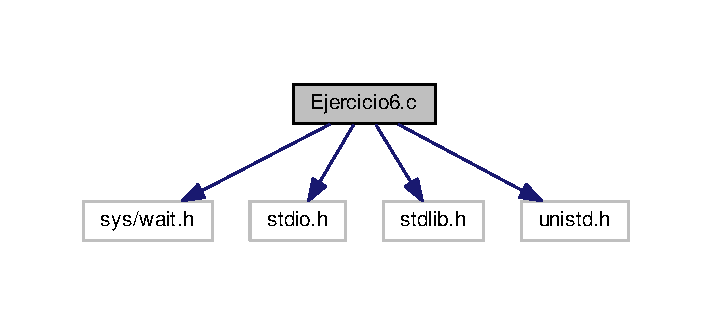
\includegraphics[width=342pt]{Ejercicio6_8c__incl}
\end{center}
\end{figure}
\subsection*{Classes}
\begin{DoxyCompactItemize}
\item 
struct \hyperlink{struct__estructura}{\+\_\+estructura}
\begin{DoxyCompactList}\small\item\em Estructura para guardar un texto aleatorio y el numero N de primos que tenemos que calcular. \end{DoxyCompactList}\end{DoxyCompactItemize}
\subsection*{Typedefs}
\begin{DoxyCompactItemize}
\item 
typedef struct \hyperlink{struct__estructura}{\+\_\+estructura} \hyperlink{Ejercicio6_8c_a958d30924884ac1bf0044585c8bc825c}{estructura}
\begin{DoxyCompactList}\small\item\em Estructura para duplicar en un proceso y su hijo. \end{DoxyCompactList}\end{DoxyCompactItemize}
\subsection*{Functions}
\begin{DoxyCompactItemize}
\item 
int \hyperlink{Ejercicio6_8c_ae66f6b31b5ad750f1fe042a706a4e3d4}{main} ()
\begin{DoxyCompactList}\small\item\em Creamos dos procesos e intentamos compartir una variable. \end{DoxyCompactList}\end{DoxyCompactItemize}


\subsection{Detailed Description}
Ejercicio 6. Ejercicio que nos permite ver el funcionamiento de la memoria y las variables entre un proceso padre y su hijo. 

\begin{DoxyAuthor}{Author}
\href{mailto:Javier.delgadod@estudiante.uam.es}{\tt Javier.\+delgadod@estudiante.\+uam.\+es} \href{mailto:Javier.lopezcano@estudiante.uam.es}{\tt Javier.\+lopezcano@estudiante.\+uam.\+es} 
\end{DoxyAuthor}


\subsection{Typedef Documentation}
\index{Ejercicio6.\+c@{Ejercicio6.\+c}!estructura@{estructura}}
\index{estructura@{estructura}!Ejercicio6.\+c@{Ejercicio6.\+c}}
\subsubsection[{\texorpdfstring{estructura}{estructura}}]{\setlength{\rightskip}{0pt plus 5cm}typedef struct {\bf \+\_\+estructura} {\bf estructura}}\hypertarget{Ejercicio6_8c_a958d30924884ac1bf0044585c8bc825c}{}\label{Ejercicio6_8c_a958d30924884ac1bf0044585c8bc825c}


Estructura para duplicar en un proceso y su hijo. 

Compuesta con un string de 80 caracteres y un entero. 

\subsection{Function Documentation}
\index{Ejercicio6.\+c@{Ejercicio6.\+c}!main@{main}}
\index{main@{main}!Ejercicio6.\+c@{Ejercicio6.\+c}}
\subsubsection[{\texorpdfstring{main()}{main()}}]{\setlength{\rightskip}{0pt plus 5cm}int main (
\begin{DoxyParamCaption}
{}
\end{DoxyParamCaption}
)}\hypertarget{Ejercicio6_8c_ae66f6b31b5ad750f1fe042a706a4e3d4}{}\label{Ejercicio6_8c_ae66f6b31b5ad750f1fe042a706a4e3d4}


Creamos dos procesos e intentamos compartir una variable. 

\hyperlink{Ejercicio6_8c_ae66f6b31b5ad750f1fe042a706a4e3d4}{main()} Reservamos memoria para una estructura y hacemos fork. Modificamos la estructura en el hijo, y cuando acaba, intentamos acceder a ella desde el padre. 
\hypertarget{Ejercicio6__dem_8c}{}\section{Ejercicio6\+\_\+dem.\+c File Reference}
\label{Ejercicio6__dem_8c}\index{Ejercicio6\+\_\+dem.\+c@{Ejercicio6\+\_\+dem.\+c}}


Demostracion de la respuesta aportada en el ejercicio 6. Queremos demostrar que al hacer fork el hijo recibe una copia exacta, pero independiente, de la informaciion que el padre tiene guardada.  


{\ttfamily \#include $<$sys/wait.\+h$>$}\\*
{\ttfamily \#include $<$stdio.\+h$>$}\\*
{\ttfamily \#include $<$stdlib.\+h$>$}\\*
{\ttfamily \#include $<$string.\+h$>$}\\*
{\ttfamily \#include $<$unistd.\+h$>$}\\*
Include dependency graph for Ejercicio6\+\_\+dem.\+c\+:
\nopagebreak
\begin{figure}[H]
\begin{center}
\leavevmode
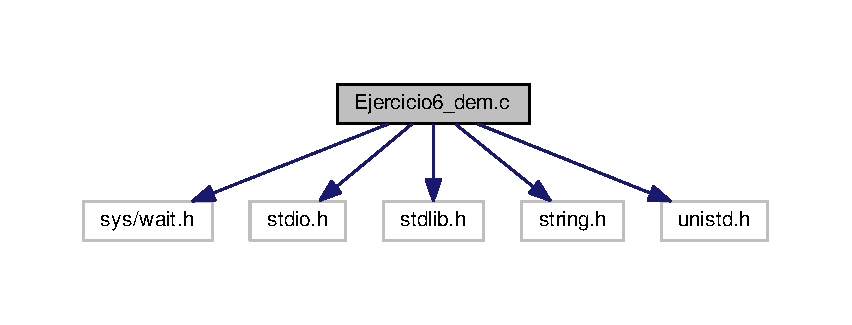
\includegraphics[width=350pt]{Ejercicio6__dem_8c__incl}
\end{center}
\end{figure}
\subsection*{Classes}
\begin{DoxyCompactItemize}
\item 
struct \hyperlink{struct__estructura}{\+\_\+estructura}
\begin{DoxyCompactList}\small\item\em Estructura para guardar un texto aleatorio y el numero N de primos que tenemos que calcular. \end{DoxyCompactList}\end{DoxyCompactItemize}
\subsection*{Typedefs}
\begin{DoxyCompactItemize}
\item 
typedef struct \hyperlink{struct__estructura}{\+\_\+estructura} \hyperlink{Ejercicio6__dem_8c_a958d30924884ac1bf0044585c8bc825c}{estructura}
\begin{DoxyCompactList}\small\item\em Estructura para duplicar en un proceso y su hijo. \end{DoxyCompactList}\end{DoxyCompactItemize}
\subsection*{Functions}
\begin{DoxyCompactItemize}
\item 
int \hyperlink{Ejercicio6__dem_8c_ae66f6b31b5ad750f1fe042a706a4e3d4}{main} ()
\begin{DoxyCompactList}\small\item\em Creamos dos procesos e intentamos compartir una variable. \end{DoxyCompactList}\end{DoxyCompactItemize}


\subsection{Detailed Description}
Demostracion de la respuesta aportada en el ejercicio 6. Queremos demostrar que al hacer fork el hijo recibe una copia exacta, pero independiente, de la informaciion que el padre tiene guardada. 

\begin{DoxyAuthor}{Author}
\href{mailto:Javier.delgadod@estudiante.uam.es}{\tt Javier.\+delgadod@estudiante.\+uam.\+es} \href{mailto:Javier.lopezcano@estudiante.uam.es}{\tt Javier.\+lopezcano@estudiante.\+uam.\+es} 
\end{DoxyAuthor}


\subsection{Typedef Documentation}
\index{Ejercicio6\+\_\+dem.\+c@{Ejercicio6\+\_\+dem.\+c}!estructura@{estructura}}
\index{estructura@{estructura}!Ejercicio6\+\_\+dem.\+c@{Ejercicio6\+\_\+dem.\+c}}
\subsubsection[{\texorpdfstring{estructura}{estructura}}]{\setlength{\rightskip}{0pt plus 5cm}typedef struct {\bf \+\_\+estructura} {\bf estructura}}\hypertarget{Ejercicio6__dem_8c_a958d30924884ac1bf0044585c8bc825c}{}\label{Ejercicio6__dem_8c_a958d30924884ac1bf0044585c8bc825c}


Estructura para duplicar en un proceso y su hijo. 

Compuesta con un string de 80 caracteres y un entero. 

\subsection{Function Documentation}
\index{Ejercicio6\+\_\+dem.\+c@{Ejercicio6\+\_\+dem.\+c}!main@{main}}
\index{main@{main}!Ejercicio6\+\_\+dem.\+c@{Ejercicio6\+\_\+dem.\+c}}
\subsubsection[{\texorpdfstring{main()}{main()}}]{\setlength{\rightskip}{0pt plus 5cm}int main (
\begin{DoxyParamCaption}
{}
\end{DoxyParamCaption}
)}\hypertarget{Ejercicio6__dem_8c_ae66f6b31b5ad750f1fe042a706a4e3d4}{}\label{Ejercicio6__dem_8c_ae66f6b31b5ad750f1fe042a706a4e3d4}


Creamos dos procesos e intentamos compartir una variable. 

\hyperlink{Ejercicio6__dem_8c_ae66f6b31b5ad750f1fe042a706a4e3d4}{main()} Reservamos memoria para una estructura y la inicializamos. Hacemos fork, cambiamos la estructura en el proceso hijo y lo acabamos. Una vez acabado el proceso hijo intenamos aceder a la informacion desde el padre, y podemos ver que el padre no puede acceder a lo modificado por el hijo. 
\hypertarget{Ejercicio8_8c}{}\section{Ejercicio8.\+c File Reference}
\label{Ejercicio8_8c}\index{Ejercicio8.\+c@{Ejercicio8.\+c}}


Ejercicio 8 de la Practica 2.  


{\ttfamily \#include $<$stdio.\+h$>$}\\*
{\ttfamily \#include $<$sys/types.\+h$>$}\\*
{\ttfamily \#include $<$sys/ipc.\+h$>$}\\*
{\ttfamily \#include $<$sys/sem.\+h$>$}\\*
{\ttfamily \#include $<$errno.\+h$>$}\\*
{\ttfamily \#include $<$sys/shm.\+h$>$}\\*
{\ttfamily \#include $<$stdlib.\+h$>$}\\*
{\ttfamily \#include \char`\"{}Ejercicio8.\+h\char`\"{}}\\*
Include dependency graph for Ejercicio8.\+c\+:
\nopagebreak
\begin{figure}[H]
\begin{center}
\leavevmode
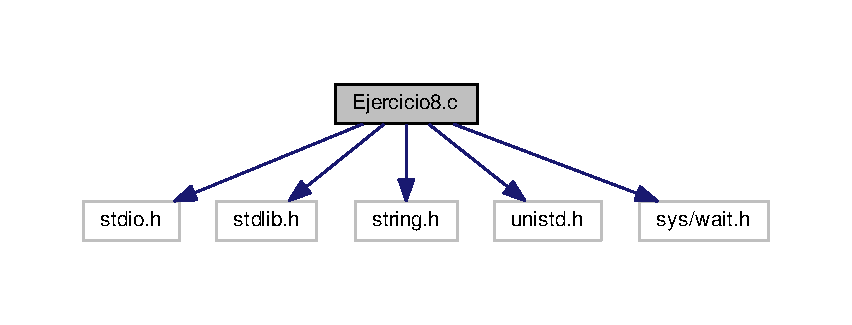
\includegraphics[width=350pt]{Ejercicio8_8c__incl}
\end{center}
\end{figure}
\subsection*{Classes}
\begin{DoxyCompactItemize}
\item 
union \hyperlink{unionsemun}{semun}
\end{DoxyCompactItemize}
\subsection*{Macros}
\begin{DoxyCompactItemize}
\item 
\#define {\bfseries S\+E\+M\+K\+EY}~75798\hypertarget{Ejercicio8_8c_ada831b9e37399bf906c8184a888e28cd}{}\label{Ejercicio8_8c_ada831b9e37399bf906c8184a888e28cd}

\item 
\#define {\bfseries N\+\_\+\+S\+E\+M\+A\+F\+O\+R\+OS}~2\hypertarget{Ejercicio8_8c_a95c81905ff3d55e62fb763f407f9fab1}{}\label{Ejercicio8_8c_a95c81905ff3d55e62fb763f407f9fab1}

\end{DoxyCompactItemize}
\subsection*{Functions}
\begin{DoxyCompactItemize}
\item 
int \hyperlink{Ejercicio8_8c_a4af104b0ed37e6ae0289a1059bc6e990}{Inicializar\+\_\+\+Semaforo} (int semid, unsigned short $\ast$array)
\begin{DoxyCompactList}\small\item\em Función que inicializa un array de semaforos con id semid y con los valores que se pasan a traves del array de shorts. \end{DoxyCompactList}\item 
int \hyperlink{Ejercicio8_8c_a731339337960a681efa435a10f12c312}{Borrar\+\_\+\+Semaforo} (int semid)
\begin{DoxyCompactList}\small\item\em Función que elimina un array de semaforos. \end{DoxyCompactList}\item 
int \hyperlink{Ejercicio8_8c_a16b16dd895b5f4cbe48f1ac8977e8b35}{Crear\+\_\+\+Semaforo} (key\+\_\+t key, int size, int $\ast$semid)
\begin{DoxyCompactList}\small\item\em Funcion que crea un array de semaforos. \end{DoxyCompactList}\item 
int \hyperlink{Ejercicio8_8c_a883244cd3b83c42cda23687da1b63369}{Down\+\_\+\+Semaforo} (int id, int num\+\_\+sem, int undo)
\begin{DoxyCompactList}\small\item\em Funcion que baja un semaforo. \end{DoxyCompactList}\item 
int \hyperlink{Ejercicio8_8c_ab375ebfc38acbdced46e062a689d5fad}{Down\+Multiple\+\_\+\+Semaforo} (int id, int size, int undo, int $\ast$active)
\begin{DoxyCompactList}\small\item\em Funcion que baja varios semaforos de un array llamando varias veces a Down\+\_\+\+Semaforo. \end{DoxyCompactList}\item 
int \hyperlink{Ejercicio8_8c_a2d5e735aecee4f493898b3d4ebab1a10}{Up\+\_\+\+Semaforo} (int id, int num\+\_\+sem, int undo)
\begin{DoxyCompactList}\small\item\em Funcion que sube un semaforo. \end{DoxyCompactList}\item 
int \hyperlink{Ejercicio8_8c_a943759695f018d64a94b8a2c49308092}{Up\+Multiple\+\_\+\+Semaforo} (int id, int size, int undo, int $\ast$active)
\begin{DoxyCompactList}\small\item\em Funcion que sube varios semaforos de un array llamando varias veces a Up\+\_\+\+Semaforo. \end{DoxyCompactList}\item 
int \hyperlink{Ejercicio8_8c_ac8da963855e09bf929c085486f4a3b47}{test} ()
\begin{DoxyCompactList}\small\item\em Programa que prueba el funcionamiento de la libreria. \end{DoxyCompactList}\end{DoxyCompactItemize}
\subsection*{Variables}
\begin{DoxyCompactItemize}
\item 
union \hyperlink{unionsemun}{semun} {\bfseries arg}\hypertarget{Ejercicio8_8c_a7c4d098a46a7276dc49238b0590c594a}{}\label{Ejercicio8_8c_a7c4d098a46a7276dc49238b0590c594a}

\end{DoxyCompactItemize}


\subsection{Detailed Description}
Ejercicio 8 de la Practica 2. 

\begin{DoxyAuthor}{Author}
\href{mailto:Javier.delgadod@estudiante.uam.es}{\tt Javier.\+delgadod@estudiante.\+uam.\+es} 

\href{mailto:Javier.lopezcano@estudiante.uam.es}{\tt Javier.\+lopezcano@estudiante.\+uam.\+es} 
\end{DoxyAuthor}


\subsection{Function Documentation}
\index{Ejercicio8.\+c@{Ejercicio8.\+c}!Borrar\+\_\+\+Semaforo@{Borrar\+\_\+\+Semaforo}}
\index{Borrar\+\_\+\+Semaforo@{Borrar\+\_\+\+Semaforo}!Ejercicio8.\+c@{Ejercicio8.\+c}}
\subsubsection[{\texorpdfstring{Borrar\+\_\+\+Semaforo(int semid)}{Borrar_Semaforo(int semid)}}]{\setlength{\rightskip}{0pt plus 5cm}int Borrar\+\_\+\+Semaforo (
\begin{DoxyParamCaption}
\item[{int}]{semid}
\end{DoxyParamCaption}
)}\hypertarget{Ejercicio8_8c_a731339337960a681efa435a10f12c312}{}\label{Ejercicio8_8c_a731339337960a681efa435a10f12c312}


Función que elimina un array de semaforos. 


\begin{DoxyParams}{Parameters}
{\em semid} & Int que es el id del array de semáforos. \\
\hline
\end{DoxyParams}
\begin{DoxyReturn}{Returns}
int que determina si la funcion se ha ejecutado o no con exito. 
\end{DoxyReturn}
\index{Ejercicio8.\+c@{Ejercicio8.\+c}!Crear\+\_\+\+Semaforo@{Crear\+\_\+\+Semaforo}}
\index{Crear\+\_\+\+Semaforo@{Crear\+\_\+\+Semaforo}!Ejercicio8.\+c@{Ejercicio8.\+c}}
\subsubsection[{\texorpdfstring{Crear\+\_\+\+Semaforo(key\+\_\+t key, int size, int $\ast$semid)}{Crear_Semaforo(key_t key, int size, int *semid)}}]{\setlength{\rightskip}{0pt plus 5cm}int Crear\+\_\+\+Semaforo (
\begin{DoxyParamCaption}
\item[{key\+\_\+t}]{key, }
\item[{int}]{size, }
\item[{int $\ast$}]{semid}
\end{DoxyParamCaption}
)}\hypertarget{Ejercicio8_8c_a16b16dd895b5f4cbe48f1ac8977e8b35}{}\label{Ejercicio8_8c_a16b16dd895b5f4cbe48f1ac8977e8b35}


Funcion que crea un array de semaforos. 


\begin{DoxyParams}{Parameters}
{\em key} & Identificador de I\+PC. \\
\hline
{\em size} & Tamano del array de semaforos que se quiere crear. \\
\hline
{\em semid} & Int que es el id del array de semáforos. \\
\hline
\end{DoxyParams}
\begin{DoxyReturn}{Returns}
int que determina si la funcion se ha ejecutado o no con exito. 
\end{DoxyReturn}
\index{Ejercicio8.\+c@{Ejercicio8.\+c}!Down\+\_\+\+Semaforo@{Down\+\_\+\+Semaforo}}
\index{Down\+\_\+\+Semaforo@{Down\+\_\+\+Semaforo}!Ejercicio8.\+c@{Ejercicio8.\+c}}
\subsubsection[{\texorpdfstring{Down\+\_\+\+Semaforo(int id, int num\+\_\+sem, int undo)}{Down_Semaforo(int id, int num_sem, int undo)}}]{\setlength{\rightskip}{0pt plus 5cm}int Down\+\_\+\+Semaforo (
\begin{DoxyParamCaption}
\item[{int}]{id, }
\item[{int}]{num\+\_\+sem, }
\item[{int}]{undo}
\end{DoxyParamCaption}
)}\hypertarget{Ejercicio8_8c_a883244cd3b83c42cda23687da1b63369}{}\label{Ejercicio8_8c_a883244cd3b83c42cda23687da1b63369}


Funcion que baja un semaforo. 


\begin{DoxyParams}{Parameters}
{\em id} & Int con el id del array de semaforos. \\
\hline
{\em num\+\_\+sem} & Int con el indice del semaforo que se quiere bajar. \\
\hline
{\em undo} & Int que es la bandera que hay que usar en la estructura sem\+\_\+oper. \\
\hline
\end{DoxyParams}
\begin{DoxyReturn}{Returns}
int que determina si la funcion se ha ejecutado o no con exito. 
\end{DoxyReturn}
\index{Ejercicio8.\+c@{Ejercicio8.\+c}!Down\+Multiple\+\_\+\+Semaforo@{Down\+Multiple\+\_\+\+Semaforo}}
\index{Down\+Multiple\+\_\+\+Semaforo@{Down\+Multiple\+\_\+\+Semaforo}!Ejercicio8.\+c@{Ejercicio8.\+c}}
\subsubsection[{\texorpdfstring{Down\+Multiple\+\_\+\+Semaforo(int id, int size, int undo, int $\ast$active)}{DownMultiple_Semaforo(int id, int size, int undo, int *active)}}]{\setlength{\rightskip}{0pt plus 5cm}int Down\+Multiple\+\_\+\+Semaforo (
\begin{DoxyParamCaption}
\item[{int}]{id, }
\item[{int}]{size, }
\item[{int}]{undo, }
\item[{int $\ast$}]{active}
\end{DoxyParamCaption}
)}\hypertarget{Ejercicio8_8c_ab375ebfc38acbdced46e062a689d5fad}{}\label{Ejercicio8_8c_ab375ebfc38acbdced46e062a689d5fad}


Funcion que baja varios semaforos de un array llamando varias veces a Down\+\_\+\+Semaforo. 


\begin{DoxyParams}{Parameters}
{\em id} & Int con el id del array de semaforos. \\
\hline
{\em size} & Int con el tamano del array de semaforos. \\
\hline
{\em undo} & Int que es la bandera que hay que usar en la estructura sem\+\_\+oper. \\
\hline
{\em active} & Array de int con los indices de los semaforos que se quiere bajar. \\
\hline
\end{DoxyParams}
\begin{DoxyReturn}{Returns}
int que determina si la funcion se ha ejecutado o no con exito. 
\end{DoxyReturn}
\index{Ejercicio8.\+c@{Ejercicio8.\+c}!Inicializar\+\_\+\+Semaforo@{Inicializar\+\_\+\+Semaforo}}
\index{Inicializar\+\_\+\+Semaforo@{Inicializar\+\_\+\+Semaforo}!Ejercicio8.\+c@{Ejercicio8.\+c}}
\subsubsection[{\texorpdfstring{Inicializar\+\_\+\+Semaforo(int semid, unsigned short $\ast$array)}{Inicializar_Semaforo(int semid, unsigned short *array)}}]{\setlength{\rightskip}{0pt plus 5cm}int Inicializar\+\_\+\+Semaforo (
\begin{DoxyParamCaption}
\item[{int}]{semid, }
\item[{unsigned short $\ast$}]{array}
\end{DoxyParamCaption}
)}\hypertarget{Ejercicio8_8c_a4af104b0ed37e6ae0289a1059bc6e990}{}\label{Ejercicio8_8c_a4af104b0ed37e6ae0289a1059bc6e990}


Función que inicializa un array de semaforos con id semid y con los valores que se pasan a traves del array de shorts. 


\begin{DoxyParams}{Parameters}
{\em semid} & Int que es el id del array de semaforos. \\
\hline
{\em array} & Array de shorts con la informacion para inicializar los semaforos. \\
\hline
\end{DoxyParams}
\begin{DoxyReturn}{Returns}
int que determina si la funcion se ha ejecutado o no con exito. 
\end{DoxyReturn}
\index{Ejercicio8.\+c@{Ejercicio8.\+c}!test@{test}}
\index{test@{test}!Ejercicio8.\+c@{Ejercicio8.\+c}}
\subsubsection[{\texorpdfstring{test()}{test()}}]{\setlength{\rightskip}{0pt plus 5cm}int test (
\begin{DoxyParamCaption}
{}
\end{DoxyParamCaption}
)}\hypertarget{Ejercicio8_8c_ac8da963855e09bf929c085486f4a3b47}{}\label{Ejercicio8_8c_ac8da963855e09bf929c085486f4a3b47}


Programa que prueba el funcionamiento de la libreria. 

\begin{DoxyReturn}{Returns}
int que determina si el programa se ha ejecutado o no con exito. 
\end{DoxyReturn}
\index{Ejercicio8.\+c@{Ejercicio8.\+c}!Up\+\_\+\+Semaforo@{Up\+\_\+\+Semaforo}}
\index{Up\+\_\+\+Semaforo@{Up\+\_\+\+Semaforo}!Ejercicio8.\+c@{Ejercicio8.\+c}}
\subsubsection[{\texorpdfstring{Up\+\_\+\+Semaforo(int id, int num\+\_\+sem, int undo)}{Up_Semaforo(int id, int num_sem, int undo)}}]{\setlength{\rightskip}{0pt plus 5cm}int Up\+\_\+\+Semaforo (
\begin{DoxyParamCaption}
\item[{int}]{id, }
\item[{int}]{num\+\_\+sem, }
\item[{int}]{undo}
\end{DoxyParamCaption}
)}\hypertarget{Ejercicio8_8c_a2d5e735aecee4f493898b3d4ebab1a10}{}\label{Ejercicio8_8c_a2d5e735aecee4f493898b3d4ebab1a10}


Funcion que sube un semaforo. 


\begin{DoxyParams}{Parameters}
{\em id} & Int con el id del array de semaforos. \\
\hline
{\em num\+\_\+sem} & Int con el indice del semaforo que se quiere subir. \\
\hline
{\em undo} & Int que es la bandera que hay que usar en la estructura sem\+\_\+oper. \\
\hline
\end{DoxyParams}
\begin{DoxyReturn}{Returns}
int que determina si la funcion se ha ejecutado o no con exito. 
\end{DoxyReturn}
\index{Ejercicio8.\+c@{Ejercicio8.\+c}!Up\+Multiple\+\_\+\+Semaforo@{Up\+Multiple\+\_\+\+Semaforo}}
\index{Up\+Multiple\+\_\+\+Semaforo@{Up\+Multiple\+\_\+\+Semaforo}!Ejercicio8.\+c@{Ejercicio8.\+c}}
\subsubsection[{\texorpdfstring{Up\+Multiple\+\_\+\+Semaforo(int id, int size, int undo, int $\ast$active)}{UpMultiple_Semaforo(int id, int size, int undo, int *active)}}]{\setlength{\rightskip}{0pt plus 5cm}int Up\+Multiple\+\_\+\+Semaforo (
\begin{DoxyParamCaption}
\item[{int}]{id, }
\item[{int}]{size, }
\item[{int}]{undo, }
\item[{int $\ast$}]{active}
\end{DoxyParamCaption}
)}\hypertarget{Ejercicio8_8c_a943759695f018d64a94b8a2c49308092}{}\label{Ejercicio8_8c_a943759695f018d64a94b8a2c49308092}


Funcion que sube varios semaforos de un array llamando varias veces a Up\+\_\+\+Semaforo. 


\begin{DoxyParams}{Parameters}
{\em id} & Int con el id del array de semaforos. \\
\hline
{\em size} & Int con el tamano del array de semaforos. \\
\hline
{\em undo} & Int que es la bandera que hay que usar en la estructura sem\+\_\+oper. \\
\hline
{\em active} & Array de int con los indices de los semaforos que se quiere subir. \\
\hline
\end{DoxyParams}
\begin{DoxyReturn}{Returns}
int que determina si la funcion se ha ejecutado o no con exito. 
\end{DoxyReturn}

\hypertarget{Ejercicio9_8c}{}\section{Ejercicio9.\+c File Reference}
\label{Ejercicio9_8c}\index{Ejercicio9.\+c@{Ejercicio9.\+c}}


Ejercicio 9. Dados dos numeros pasados en la entrada, calculamos el factorial de uno partido del otro, uno elevado al otro, la suma con valores absolutos y el numero combinatorio de uno sobre todo. Cada operacion se realiza en un proceso distinto, que se comunica con el padre mediante pipes.  


{\ttfamily \#include $<$stdio.\+h$>$}\\*
{\ttfamily \#include $<$stdlib.\+h$>$}\\*
{\ttfamily \#include $<$math.\+h$>$}\\*
{\ttfamily \#include $<$unistd.\+h$>$}\\*
{\ttfamily \#include $<$string.\+h$>$}\\*
{\ttfamily \#include $<$sys/wait.\+h$>$}\\*
{\ttfamily \#include $<$sys/types.\+h$>$}\\*
Include dependency graph for Ejercicio9.\+c\+:
\nopagebreak
\begin{figure}[H]
\begin{center}
\leavevmode
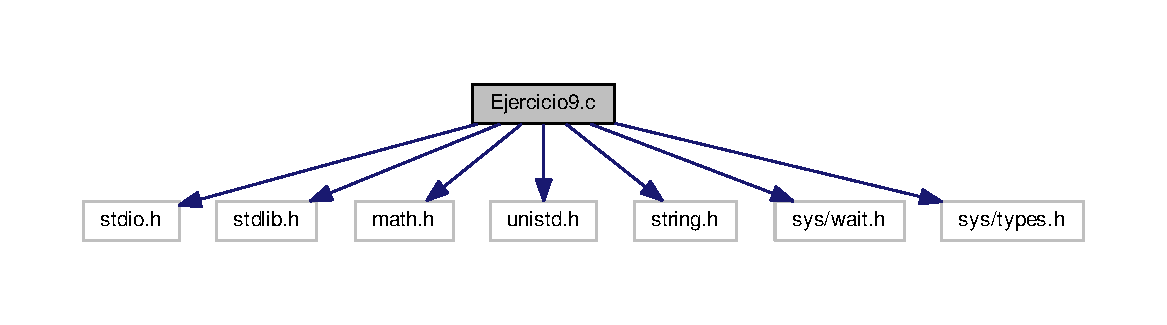
\includegraphics[width=350pt]{Ejercicio9_8c__incl}
\end{center}
\end{figure}
\subsection*{Functions}
\begin{DoxyCompactItemize}
\item 
double \hyperlink{Ejercicio9_8c_a1e86e884e71a85fdafe94dc3ee7f77f8}{potencia} (int a, int b)
\begin{DoxyCompactList}\small\item\em hacemos la operacion matematica a$^\wedge$b \end{DoxyCompactList}\item 
double \hyperlink{Ejercicio9_8c_a5cf432a7c889fe75dffc281247cb867e}{factorial} (int a, int b)
\begin{DoxyCompactList}\small\item\em hacemos la operacion matematica a!/b \end{DoxyCompactList}\item 
double \hyperlink{Ejercicio9_8c_ab13db5a54377e7e55eb6db91185af27e}{num\+Combinatorio} (int a, int b)
\begin{DoxyCompactList}\small\item\em hallamos el numero combinatorio a sobre b de forma recursiva \end{DoxyCompactList}\item 
double \hyperlink{Ejercicio9_8c_a7d7edaebcf72f07f2ca29c75e69460e1}{suma\+Absoluta} (int a, int b)
\begin{DoxyCompactList}\small\item\em hallamos la suma de a y b en valores absolutos \end{DoxyCompactList}\item 
int \hyperlink{Ejercicio9_8c_ae66f6b31b5ad750f1fe042a706a4e3d4}{main} ()
\begin{DoxyCompactList}\small\item\em Hacemos distintas operaciones matemáticas sobre dos numeros en procesos independientes. \end{DoxyCompactList}\end{DoxyCompactItemize}


\subsection{Detailed Description}
Ejercicio 9. Dados dos numeros pasados en la entrada, calculamos el factorial de uno partido del otro, uno elevado al otro, la suma con valores absolutos y el numero combinatorio de uno sobre todo. Cada operacion se realiza en un proceso distinto, que se comunica con el padre mediante pipes. 

\begin{DoxyAuthor}{Author}
\href{mailto:Javier.delgadod@estudiante.uam.es}{\tt Javier.\+delgadod@estudiante.\+uam.\+es} \href{mailto:Javier.lopezcano@estudiante.uam.es}{\tt Javier.\+lopezcano@estudiante.\+uam.\+es} 
\end{DoxyAuthor}


\subsection{Function Documentation}
\index{Ejercicio9.\+c@{Ejercicio9.\+c}!factorial@{factorial}}
\index{factorial@{factorial}!Ejercicio9.\+c@{Ejercicio9.\+c}}
\subsubsection[{\texorpdfstring{factorial(int a, int b)}{factorial(int a, int b)}}]{\setlength{\rightskip}{0pt plus 5cm}double factorial (
\begin{DoxyParamCaption}
\item[{int}]{a, }
\item[{int}]{b}
\end{DoxyParamCaption}
)}\hypertarget{Ejercicio9_8c_a5cf432a7c889fe75dffc281247cb867e}{}\label{Ejercicio9_8c_a5cf432a7c889fe75dffc281247cb867e}


hacemos la operacion matematica a!/b 

\hyperlink{Ejercicio9_8c_a5cf432a7c889fe75dffc281247cb867e}{factorial(int a, int b)} hacemos factorial 
\begin{DoxyParams}{Parameters}
{\em a} & numero sobre el que hacemos el factorial \\
\hline
{\em b} & cociente de la opercion \\
\hline
\end{DoxyParams}
\begin{DoxyReturn}{Returns}
double a!/b 
\end{DoxyReturn}
\index{Ejercicio9.\+c@{Ejercicio9.\+c}!main@{main}}
\index{main@{main}!Ejercicio9.\+c@{Ejercicio9.\+c}}
\subsubsection[{\texorpdfstring{main()}{main()}}]{\setlength{\rightskip}{0pt plus 5cm}int main (
\begin{DoxyParamCaption}
{}
\end{DoxyParamCaption}
)}\hypertarget{Ejercicio9_8c_ae66f6b31b5ad750f1fe042a706a4e3d4}{}\label{Ejercicio9_8c_ae66f6b31b5ad750f1fe042a706a4e3d4}


Hacemos distintas operaciones matemáticas sobre dos numeros en procesos independientes. 

Creamos cuatro procesos y ocho pipes (una de escritura y otra de lectura para cada proceso), de forma que desde el padre enviamos los dos operandos y desde los hijos los resultados para que el padre los imprima.

\begin{DoxyReturn}{Returns}
int que determina si el programa se ha ejecutado o no con exito. 
\end{DoxyReturn}
\index{Ejercicio9.\+c@{Ejercicio9.\+c}!num\+Combinatorio@{num\+Combinatorio}}
\index{num\+Combinatorio@{num\+Combinatorio}!Ejercicio9.\+c@{Ejercicio9.\+c}}
\subsubsection[{\texorpdfstring{num\+Combinatorio(int a, int b)}{numCombinatorio(int a, int b)}}]{\setlength{\rightskip}{0pt plus 5cm}double num\+Combinatorio (
\begin{DoxyParamCaption}
\item[{int}]{a, }
\item[{int}]{b}
\end{DoxyParamCaption}
)}\hypertarget{Ejercicio9_8c_ab13db5a54377e7e55eb6db91185af27e}{}\label{Ejercicio9_8c_ab13db5a54377e7e55eb6db91185af27e}


hallamos el numero combinatorio a sobre b de forma recursiva 

\hyperlink{Ejercicio9_8c_a5cf432a7c889fe75dffc281247cb867e}{factorial(int a, int b)} hacemos el numero combinatorio a sobre b 
\begin{DoxyParams}{Parameters}
{\em a} & numero de elementos del conjunto \\
\hline
{\em b} & numero de elementos a escoger del conjunto \\
\hline
\end{DoxyParams}
\begin{DoxyReturn}{Returns}
double numero combinatorio a sobre b 
\end{DoxyReturn}
\index{Ejercicio9.\+c@{Ejercicio9.\+c}!potencia@{potencia}}
\index{potencia@{potencia}!Ejercicio9.\+c@{Ejercicio9.\+c}}
\subsubsection[{\texorpdfstring{potencia(int a, int b)}{potencia(int a, int b)}}]{\setlength{\rightskip}{0pt plus 5cm}double potencia (
\begin{DoxyParamCaption}
\item[{int}]{a, }
\item[{int}]{b}
\end{DoxyParamCaption}
)}\hypertarget{Ejercicio9_8c_a1e86e884e71a85fdafe94dc3ee7f77f8}{}\label{Ejercicio9_8c_a1e86e884e71a85fdafe94dc3ee7f77f8}


hacemos la operacion matematica a$^\wedge$b 

\hyperlink{Ejercicio9_8c_a1e86e884e71a85fdafe94dc3ee7f77f8}{potencia(int a, int b)} hacemos a$^\wedge$b 
\begin{DoxyParams}{Parameters}
{\em a} & base de la operacion \\
\hline
{\em b} & exponente de la operacion \\
\hline
\end{DoxyParams}
\begin{DoxyReturn}{Returns}
double a$^\wedge$b 
\end{DoxyReturn}
\index{Ejercicio9.\+c@{Ejercicio9.\+c}!suma\+Absoluta@{suma\+Absoluta}}
\index{suma\+Absoluta@{suma\+Absoluta}!Ejercicio9.\+c@{Ejercicio9.\+c}}
\subsubsection[{\texorpdfstring{suma\+Absoluta(int a, int b)}{sumaAbsoluta(int a, int b)}}]{\setlength{\rightskip}{0pt plus 5cm}double suma\+Absoluta (
\begin{DoxyParamCaption}
\item[{int}]{a, }
\item[{int}]{b}
\end{DoxyParamCaption}
)}\hypertarget{Ejercicio9_8c_a7d7edaebcf72f07f2ca29c75e69460e1}{}\label{Ejercicio9_8c_a7d7edaebcf72f07f2ca29c75e69460e1}


hallamos la suma de a y b en valores absolutos 

\hyperlink{Ejercicio9_8c_a5cf432a7c889fe75dffc281247cb867e}{factorial(int a, int b)} hacemos el numero combinatorio a sobre b 
\begin{DoxyParams}{Parameters}
{\em a} & primer operando \\
\hline
{\em b} & segundo operando \\
\hline
\end{DoxyParams}
\begin{DoxyReturn}{Returns}
double valor absoluto de a mas valor absoluto de b 
\end{DoxyReturn}

%--- End generated contents ---

% Index
\backmatter
\newpage
\phantomsection
\clearemptydoublepage
\addcontentsline{toc}{chapter}{Index}
\printindex

\end{document}
